\باب{ترچھی آمد، انعکاس، انحراف اور  انکسار}
دو خطوں کے سرحد پر عمودی آمدی موج کے انعکاس اور ترسیل پر باب \حوالہ{باب_مستوی_امواج} میں غور کیا گیا۔اس باب میں ترچھی آمدی موج کی بات کرتے ہوئے انعکاس اور ترسیل کے علاوہ انحراف اور انکسار کی بھی بات کی جائے گی۔عمودی امواج اور ترسیلی تار کے مساوات ہوبہو ایک جیسے تھے۔ ترچھی آمدی موج کی مساوی مثال ترسیلی تار میں نہیں پائی جاتی۔یہی وجہ ہے کہ ان پر یہاں علیحدہ  سے غور کیا جا رہا ہے۔

\حصہ{ترچھی آمد}
\جزوحصہء{عمودی قطبی برقی موج \عددیء{\kvec{E}_{\perp}}}
شکل \حوالہ{شکل_ترچھی_آمد_متوازی_برقی_میدان_عمومی_شکل} میں سرحد پر ترچھی آمد موج دکھائی گئی ہے۔دو خطوں کا سرحد \عددیء{y=0} سطح پر پایا جاتا ہے لہٰذا \عددیء{y} محدد، سرحد کے عمودی ہے۔پہلے خطے (خطہ-1) میں آمدی برقی موج کے حرکت کی سمت \عددیء{y} محدد کے ساتھ \عددیء{\theta_i} \اصطلاح{زاویہ آمد}\فرہنگ{زاویہ!آمد}\حاشیہب{incidence angle}\فرہنگ{angle!incidence} بناتی ہے جبکہ اسی خطے میں انعکاسی برقی موج کے حرکت کی سمت  \عددیء{y} محدد کے ساتھ \عددیء{\theta_r} \اصطلاح{زاویہ انعکاس}\فرہنگ{زاویہ!انعکاس}\حاشیہب{reflection angle}\فرہنگ{angle!reflection} بناتی ہے۔ترسیلی موج کے حرکت کی سمت  دوسرے خطے (خطہ-2) میں منفی \عددیء{y} محدد کے ساتھ \عددیء{\theta_t} زاویہ بناتی ہے۔ترسیلی موج کو انحرافی موج بھی کہا جاتا ہے لہٰذا \عددیء{\theta_t} \اصطلاح{زاویہ انحراف}\فرہنگ{زاویہ!انحراف}\حاشیہب{refraction angle}\فرہنگ{angle!refraction} کہلاتی ہے۔پہلے خطے کے مستقل \عددیء{\epsilon_1, \mu_1, \sigma_1} جبکہ دوسرے خطے کے مستقل \عددیء{\epsilon_2, \mu_2, \sigma_2} ہیں۔
\begin{figure}
\centering
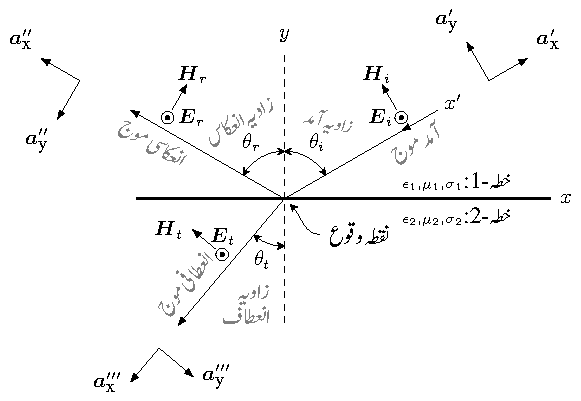
\includegraphics{figObliqueIncidencePerpendicularElectricField}
\caption{ترچھی آمد کی صورت میں انعکاسی اور ترسیلی امواج اور ان کے زاویے۔برقی میدان عمودی قطبیت رکھتی ہے۔}
\label{شکل_ترچھی_آمد_متوازی_برقی_میدان_عمومی_شکل}
\end{figure}

ہم دو صورتوں پر باری باری غور کریں گے۔ پہلی صورت میں خطی قطبی برقی میدان، سطح آمد (یعنی $xy$ سطح) کے  عمودی ہو گا جبکہ دوسری صورت میں خطی قطبی برقی میدان اس سطح کے متوازی ہو گا۔ان دو صورتوں میں برقی و مقناطیسی موج بالترتیب \اصطلاح{عمودی قطب موج}\فرہنگ{عمودی قطب موج}\فرہنگ{قطبیت!عمودی}\حاشیہب{perpendicular polarized}\فرہنگ{polarized!perpendicular} اور \اصطلاح{متوازی قطب موج}\فرہنگ{متوازی قطب موج}\فرہنگ{قطبیت!متوازی}\حاشیہب{parallel polarized}\فرہنگ{polarized!parallel} کہلائیں گے۔شکل \حوالہ{شکل_ترچھی_آمد_متوازی_برقی_میدان_عمومی_شکل} عمودی قطبیت کی صورت حال دکھا رہی ہے۔کسی بھی عمومی برقی موج کو عمودی اور متوازی قطب کے امواج کا مجموعہ لکھا جا سکتا ہے۔

ہم دیکھ چکے ہیں کہ منفی \عددیء{z} سمت میں حرکت کرتی \عددیء{\ax} میدان کی برقی موج
\begin{align*}
\kvec{E}_i=E_0 \ax e^{j(\omega t +\beta_1 z)}
\end{align*} 
لکھی جاتی ہے۔اس موج میں برقی میدان ہر نقطے پر تمام اوقات \عددیء{\ax} سمت میں ہو گا جبکہ حرکت کی سمت منفی \عددیء{z} جانب ہے۔اب \عددیء{\ax} اکائی سمتیہ کی جگہ کسی بھی عمومی اکائی سمتیہ \عددیء{\kvec{a}} سمت کا میدان جو \عددیء{z} محدد کی بجائے لکیر \عددیء{l} پر منفی سمت کی جانب حرکت کر رہا ہو، کی موج
\begin{align*}
\kvec{E}_i=E_0 \kvec{a} e^{j(\omega t +\beta_1 l)}
\end{align*} 
لکھی جائے گی۔اب شکل \حوالہ{شکل_ترچھی_آمد_متوازی_برقی_میدان_عمومی_شکل} میں \عددیء{\kvec{E}_i} پر دوبارہ غور کریں۔یہ میدان \عددی{x'} پر منفی سمت میں حرکت کر رہی ہے جبکہ برقی میدان \عددی{\kvec{E}_i} کی سمت \عددیء{\az} ہے  لہٰذا اس موج کو
\begin{align}\label{مساوات_ترچھا_آمد_ترچھی_کارتیسی}
\kvec{E}_i=E_0 \az e^{j(\omega t +\beta_1 x')}
\end{align}
لکھا جا سکتا ہے جہاں کارتیسی محدد \عددیء{x,y} کے مرکز سے لکیر \عددیء{x'} پر فاصلہ ناپا گیا ہے۔آئیں مساوات \حوالہ{مساوات_ترچھا_آمد_ترچھی_کارتیسی} میں لکیر \عددیء{x'} پر فاصلے کو کارتیسی محدد \عددیء{x,y} کے متغیرات استعمال کرتے ہوئے ناپیں۔
%
\begin{figure}
\centering
\begin{subfigure}{0.4\textwidth}
\centering
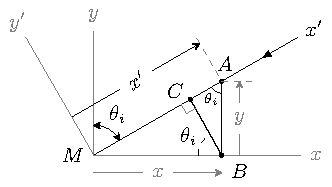
\includegraphics{figObliqueIncidencePerpendicularElectricFieldCoordinateTransformation}
\caption{فاصلے کا کارتیسی محدد میں اظہار۔}
\label{شکل_ترچھی_محدد_کی_تبدیلی}
\end{subfigure}
\begin{subfigure}{0.4\textwidth}
\centering
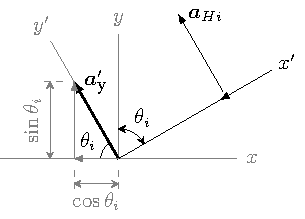
\includegraphics{figObliqueIncidencePerpendicularElectricFieldUnitVectorTransformation}
\caption{اکائی سمتیہ کا کارتیسی محدد میں اظہار۔}
\label{شکل_ترچھی_اکائی_سمتیہ}
\end{subfigure}
\caption{کسی بھی سمت میں فاصلے اور اکائی سمتیہ کو کارتیسی محدد میں لکھنے کا طریقہ۔}
\label{شکل_ترچھی_تبادلہ_فاصلہ_اور_اکائی_سمتیہ}
\end{figure}

شکل \حوالہ{شکل_ترچھی_تبادلہ_فاصلہ_اور_اکائی_سمتیہ}-الف میں آمد موج اور محدد \عددی{xy} دوبارہ دکھائے گئے ہیں۔اس شکل میں لکیر \عددیء{x'} کو محدد \عددیء{x'y'} کا حصہ دکھایا گیا ہے۔ان دونوں محدد کا مرکز نقطہ \عددی{M} ہے۔لکیر \عددیء{x'} پر نقطہ \عددیء{A} کا مرکز سے فاصلہ \عددیء{MA} کو \عددیء{x'} لکھا گیا ہے۔ اب \عددیء{MA=MC+CA} کے برابر ہے جہاں \عددیء{{MC=x \sin \theta_i}} اور \عددیء{{CA=y \cos \theta_i}} کے برابر ہیں لہٰذا
\begin{align}\label{مساوات_ترچھی_ترچھی_محدد_ایکس_کو_سیدھے_محدد_میں_لکھنا}
x'=x\sin \theta_i +y \cos \theta_i
\end{align} 
لکھا جا سکتا ہے جس سے ہم مساوات \حوالہ{مساوات_ترچھا_آمد_ترچھی_کارتیسی} کو
\begin{align}\label{مساوات_ترچھی_عمودی_برقی_آمدی}
\kvec{E}_i=E_0 \az e^{j[\omega t +\beta_1 (x\sin \theta_i +y \cos \theta_i)]}
\end{align}
لکھ سکتے ہیں۔اس مساوات میں موج  گھٹتے \عددیء{x'} کی طرف رواں ہے۔

آمدی موج کی بات کرتے ہوئے کارتیسی محدد \عددی{x'y'} کا سہارا لیا جاتا ہے  جس کے اکائی سمتیات \عددی{\ax'} اور \عددی{\ay'} کو  شکل \حوالہ{شکل_ترچھی_آمد_متوازی_برقی_میدان_عمومی_شکل} میں لکیر \عددی{x'} کے قریب دکھایا گیا ہے۔اسی طرح  انعکاسی موج پر غور کے دوران  کارتیسی محدد \عددی{x''y''} اور ترسیلی موج میں \عددی{x'''y'''} کا سہارا لیا جاتا ہے۔ان کے اکائی سمتیات کو بالترتیب  انعکاسی اور ترسیلی امواج کے قریب شکل \حوالہ{شکل_ترچھی_آمد_متوازی_برقی_میدان_عمومی_شکل} میں دکھایا گیا ہے۔ان تینوں محدد کے مرکز نقطہ \عددی{M} پر پائے جاتے ہیں۔

آمدی برقی اور مقناطیسی میدان \عددیء{x'} کے عمودی ہیں۔برقی میدان کی سمت \عددیء{\az} (یا $\az'$) ہے جہاں \عددیء{\az} اور \عددیء{\az'} دونوں ایک ہی سمت کو ظاہر کرتے ہیں۔مقناطیسی میدان \عددیء{\kvec{H}_i}  کی اکائی سمتیہ \عددیء{\kvec{a}_{Hi}} محدد \عددیء{y'}  کی سمت میں ہے۔یوں \عددیء{\kvec{a}_{Hi}=\kvec{a}_y'}  لکھا جا سکتا ہے۔آئیں \عددیء{\ay'} کو کارتیسی محدد \عددیء{x,y} کے متغیرات کی صورت میں شکل \حوالہ{شکل_ترچھی_تبادلہ_فاصلہ_اور_اکائی_سمتیہ}-ب کی مدد سے لکھیں۔اکائی سمتیہ \عددیء{\ay'} کو دو سمتیوں کے مجموعے کے طور پر دکھایا گیا ہے۔چونکہ اکائی سمتیہ کی لمبائی ایک کے برابر ہوتی ہے لہٰذا شکل میں تکون کے وتر کی لمبائی اکائی ہے۔یوں  تکون کا قاعدہ \عددیء{\cos \theta_i} اور اس کا عمود \عددیء{\sin \theta_i} کے برابر ہوں گے جس سے
\begin{align}\label{مساوات_ترچھی_اکائی_وائے_ڈیش}
\ay'=-\cos \theta_i \ax+\sin \theta_i \ay
\end{align} 
لکھا جا سکتا ہے۔ان معلومات کو استعمال کرتے ہوئے آمدی مقناطیسی موج
\begin{align*}
\kvec{H}_i&=\frac{E_0}{\eta_1} \ay' e^{j(\omega t +\beta_1 x')}
\end{align*}
کو
\begin{align}\label{مساوات_ترچھی_عمودی_برقی_میں_مقناطیسی_آمدی}
\kvec{H}_i=\frac{E_0}{\eta_1} (-\cos \theta_i \ax+\sin \theta_i \ay) e^{j[\omega t +\beta_1 (x\sin \theta_i +y \cos \theta_i)]}
\end{align}
لکھا جا سکتا ہے۔

مساوات \حوالہ{مساوات_ترچھی_عمودی_برقی_آمدی} اور مساوات \حوالہ{مساوات_ترچھی_عمودی_برقی_میں_مقناطیسی_آمدی} کے مساوی دوری سمتی مساوات مندرجہ ذیل ہیں۔
\begin{align}
\kvec{E}_{si} & = \az E_0 e^{j\beta_1 (x\sin \theta_i +y \cos \theta_i)} \label{مساوات_ترچھی_آمدی_برقی_میدان_دوری_سمتی}\\
\kvec{H}_{si} & = (-\cos \theta_i \ax+\sin \theta_i \ay)\frac{E_0}{\eta_1} e^{j\beta_1 (x\sin \theta_i +y \cos \theta_i)} \label{مساوات_ترچھی_آمدی_مقناطیسی_میدان_دوری_سمتی}
\end{align}

مساوات \حوالہ{مساوات_موج_شرح_انعکاس_تعریف} شرح انعکاس جبکہ مساوات \حوالہ{مساوات_موج_شرح_ترسیل_تعریف} شرح ترسیل کی تعریف بیان کرتے ہیں۔عین سرحد پر عمودی \عددیء{(\perp)} قطب کے میدان کے لئے ان مساوات کو
\begin{gather}
\begin{aligned}\label{مساوات_ترچھی_سرحدی_شرائط}
\Gamma_{\perp}&=\frac{E_r}{E_i} \\
\tau_{\perp} &=\frac{E_t}{E_i}
\end{aligned}
\end{gather}
لکھا جائے گا۔
\begin{figure}
\centering
\begin{subfigure}{0.4\textwidth}
\centering
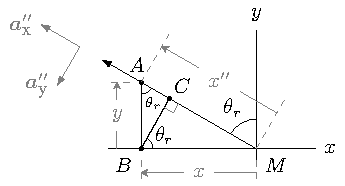
\includegraphics{figObliqueIncidencePerpendicularElectricFieldCoordinateTransformationReflecTedWave}
\caption{انعکاسی موج کے فاصلے کی کارتیسی محدد میں اظہار۔}
\label{شکل_ترچھی_انعکاسی_برقی}
\end{subfigure}%
\begin{subfigure}{0.4\textwidth}
\centering
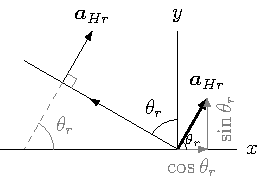
\includegraphics{figObliqueIncidencePerpendicularElectricFieldUnitMagneticVectorTransformation}
\caption{انعکاسی مقناطیسی موج کی اکائی سمتیہ کا کارتیسی محدد میں اظہار۔}
\label{شکل_ترچھی_انعکاسی_مقناطیسی_اکائی}
\end{subfigure}%
\caption{انعکاسی موج کے متغیرات کا کارتیسی محدد میں اظہار۔}
\label{شکل_ترچھی_اکائی_اظہار}
\end{figure}

شکل \حوالہ{شکل_ترچھی_اکائی_اظہار}-الف میں صرف انعکاسی  موج دکھائی گئی ہے۔مرکز \عددیء{M} سے موج کا فاصلہ \عددیء{x''} لیتے ہوئے برقی موج کی مساوات حاصل کرتے ہیں۔اب \عددیء{{MA=MC+CA}} کے برابر ہے جہاں \عددیء{{MC=-x \sin \theta_r}} اور \عددیء{{CA=y \cos \theta_r}} کے برابر ہیں لہٰذا
\begin{align}
x''=-x \sin \theta_r+y\cos \theta_r
\end{align}
لکھا جائے گا۔چونکہ منفی محدد پر \عددیء{x} کی قیمت منفی ہو گی لہٰذا \عددیء{MC} حاصل کرتے وقت منفی علامت کی ضرورت ہو گی۔یوں مثبت \عددی{x''} سمت میں حرکت کرتی  انعکاسی برقی موج
\begin{gather}
\begin{aligned} \label{مساوات_ترچھی_انعکاسی_برقی_میدان_دوری_سمتی}
\kvec{E}_{sr}&=\az \Gamma_{\perp} E_0 e^{- j \beta_1 x''}\\
&=\az \Gamma_{\perp} E_0 e^{- j \beta_1 (-x \sin \theta_r+y\cos \theta_r)}
\end{aligned}
\end{gather}
لکھی جائے گی جہاں میدان کی سمت \عددی{\az''} یعنی \عددیء{\az} ہے۔

انعکاسی مقناطیسی موج کی مساوات لکھنے کی خاطر مقناطیسی میدان کی اکائی سمتیہ درکار ہے۔شکل \حوالہ{شکل_ترچھی_اکائی_اظہار}-ب میں انعکاسی مقناطیسی میدان کی سمت میں اکائی سمتیہ \عددیء{\kvec{a}_H} دکھائی گئی ہے جو \عددیء{x} محدد کے ساتھ \عددیء{\theta_r} زاویہ بناتی ہے۔اکائی سمتیہ کو محدد کے مرکز پر دو سمتیات کے مجموعے کے طور پر بھی دکھایا گیا ہے جہاں سے
\begin{align}
\kvec{a}_{Hr}=\cos \theta_r \ax+\sin \theta_r \ay
\end{align}
لکھا جا سکتا ہے لہٰذا انعکاسی مقناطیسی موج
\begin{align} \label{مساوات_ترچھی_انعکاسی_مقناطیسی_میدان_دوری_سمتی}
\kvec{H}_{sr}=(\cos \theta_r \ax+\sin \theta_r \ay)\Gamma_{\perp} \frac{ E_0}{\eta_1} e^{-j \beta_1 (-x \sin \theta_r+y\cos \theta_r)}
\end{align}
لکھی جا سکتی ہے۔شکل سے واضح ہے کہ \عددی{\kvec{a}_{Hr}=-\ay''} ہے۔

یہی طریقہ کار استعمال  کرتے ہوئے ترسیلی امواج کے مساوات یوں لکھے جا سکتے ہیں
\begin{align}
\kvec{E}_{st} &=\az \tau_{\perp} E_0 e^{j \beta_2 (x \sin \theta_t+y\cos \theta_t)}  \label{مساوات_ترچھی_انحرافی_برقی_میدان_دوری_سمتی}\\
\kvec{H}_{st} &=(-\cos \theta_t \ax+\sin \theta_t \ay ) \tau_{\perp} \frac{E_0}{\eta_2} e^{j \beta_2 (x \sin \theta_t+y\cos \theta_t)}  \label{مساوات_ترچھی_انحرافی_مقناطیسی_میدان_دوری_سمتی}
\end{align}
جہاں ترسیلی امواج کارتیسی محدد کے مرکز سے بڑھتے فاصلے کی طرف رواں ہیں۔یہاں غور کریں کہ دوسرے خطے میں امواج کے مساوات میں مستقل \عددیء{\beta_2} اور \عددیء{\eta_2} استعمال کئے گئے ہیں۔

صفحہ \حوالہصفحہ{مساوات_میکس_ویل_سرحدی_شرائط_بدلتے_میدان_الف} پر مساوات \حوالہ{مساوات_میکس_ویل_سرحدی_شرائط_بدلتے_میدان_الف} برقی میدان کی سرحدی شرط پیش کرتی ہے جس کے مطابق سرحد کے دونوں اطراف متوازی برقی میدان برابر ہوں گے۔ برقی میدان کی شرط مساوات \حوالہ{مساوات_ترچھی_آمدی_برقی_میدان_دوری_سمتی}، مساوات \حوالہ{مساوات_ترچھی_انعکاسی_برقی_میدان_دوری_سمتی} اور  مساوات \حوالہ{مساوات_ترچھی_انحرافی_برقی_میدان_دوری_سمتی} میں \عددیء{y=0} پر کرتے ہوئے یوں
\begin{align*}
\az E_0 e^{j\beta_1 (x\sin \theta_i +0 \cos \theta_i)} +\az \Gamma_{\perp} E_0 e^{- j \beta_1 (-x \sin \theta_r+0\cos \theta_r)} =\az \tau_{\perp} E_0 e^{j \beta_2 (x \sin \theta_t+0\cos \theta_t)}
\end{align*}
یا  
\begin{align}\label{مساوات_ترچھی_انعکاسی-شرط_الف}
e^{j\beta_1 x\sin \theta_i} +\Gamma_{\perp}  e^{ j \beta_1 x \sin \theta_r} = \tau_{\perp}  e^{j \beta_2 x \sin \theta_t} 
\end{align}
لکھی جا سکتی ہے۔یہ مساوات کسی بھی \عددیء{x} کے لئے درست ہے لہٰذا یہ \عددیء{x=0} کے لئے بھی درست ہو گی۔اس میں \عددیء{x=0} پر کرنے سے
 \begin{align}\label{مساوات_ترچھی_انعکاسی-شرط_ب}
1+\Gamma_{\perp}=\tau_{\perp}
\end{align}
ملتا ہے۔مساوات \حوالہ{مساوات_ترچھی_انعکاسی-شرط_الف} میں \عددیء{x} کی قیمت تبدیل کرنے سے \عددیء{e} کے طاقت تبدیل ہوتے ہیں۔یوں یہ مساوات صرف اور صرف اس صورت \عددیء{x} کے ہر قیمت کے لئے درست ہو گی جب مساوات میں تینوں \عددیء{e} کے طاقت ہر صورت برابر ہوں یعنی 
\begin{align}
e^{j\beta_1 x\sin \theta_i}=e^{j \beta_1 x \sin \theta_r}=e^{j \beta_2 x \sin \theta_t}
\end{align}
اب پہلی دو اجزاء کے مساوات سے
\begin{align}\label{مساوات_ترچھی_زاویہ_آمد_برابر_زاویہ_انعکاس}
\theta_i=\theta_r
\end{align}
اور آخری دو اجزاء کی مساوات سے
\begin{align}\label{مساوات_ترچھی_ابن_سھل_الف}
\beta_2 \sin \theta_t= \beta_1\sin \theta_r
\end{align}
ملتا ہے جس میں مساوات \حوالہ{مساوات_ترچھی_زاویہ_آمد_برابر_زاویہ_انعکاس} پر کرتے ہوئے
\begin{align}\label{مساوات_ترچھی_عمومی_ابن_سھل}
\frac{\sin \theta_t}{\sin \theta_i}= \frac{\beta_1}{\beta_2}\quad \quad \text{\RL{قانون ابن سھل کی عمومی مساوات}}
\end{align}
حاصل ہوتا ہے۔یہ صفحہ \حوالہصفحہ{مساوات_موج_کامل-ذوبرق_بیٹا} پر دیے، بے ضیاع خطے کی مساوات \حوالہ{مساوات_موج_کامل-ذوبرق_بیٹا} پر کرنے سے
\begin{align}\label{مساوات_ترچھی_ابن_سھل_پہلی_مساوات}
\sin \theta_t &=\frac{\omega \sqrt{\mu_1 \epsilon_1}}{\omega \sqrt{\mu_2 \epsilon_2 }}\sin \theta_i =\frac{\sqrt{\mu_1 \epsilon_1}}{\sqrt{\mu_2 \epsilon_2 }}\sin \theta_i 
\end{align}
یعنی
\begin{gather}
\begin{aligned}\label{مساوات_ترچھی_انحراف}
\sin \theta_t &=\frac{\sqrt{\mu_{r1} \mu_0 \epsilon_{r1} \epsilon_0}}{ \sqrt{\mu_{r2} \mu_0 \epsilon_{r2} \epsilon_0}}\sin \theta_i \\
&=\frac{\sqrt{\mu_{r1} \epsilon_{r1}}}{\sqrt{\mu_{r2} \epsilon_{r2} }}\sin \theta_i  \quad \quad \text{\RL{قانون ابن سھل، بے ضیاع مقناطیسی خطے}}
\end{aligned}
\end{gather}
حاصل ہوتا ہے۔

غیر مقناطیسی اور بے ضیاع خطے میں بصری امواج پر تبصرے کے دوران عموماً  \اصطلاح{انحرافی مستقل}\فرہنگ{انحرافی مستقل}\فرہنگ{مستقل!انحرافی}\حاشیہب{index of refraction}\فرہنگ{refraction index} \عددی{n} استعمال کیا جاتا ہے جہاں
\begin{align*}
\sqrt{\epsilon_R}=n
\end{align*}
کے برابر ہے۔بے ضیاع، غیر مقناطیسی خطے میں مساوات \حوالہ{مساوات_ترچھی_انحراف} کو 
\begin{align}\label{مساوات_ترچھی_سنیل_قانون}
\sin \theta_t= \frac{n_1}{n_2}\sin \theta_i \quad \quad \text{\RL{قانون ابن سھل، بے ضیاع غیر مقناطیسی خطے}}
\end{align}
لکھا جا سکتا ہے جہاں
\begin{gather}
\begin{aligned}
n_1&=\sqrt{ \epsilon_{r1}}\\
n_2&=\sqrt{ \epsilon_{r2}}
\end{aligned}
\end{gather}
غیر مقناطیسی خطوں کے انحرافی مستقل ہیں۔انحرافی مستقل کو استعمال کرتے ہوئے، بے ضیاع اور غیر مقناطیسی خطے میں
\begin{align}
\beta&=\omega \sqrt{\mu \epsilon}=\omega \sqrt{\mu_0 \epsilon_0} \sqrt{\epsilon_R}=\frac{\omega n}{c}\\
\eta&=\sqrt{\frac{\mu}{\epsilon}}=\frac{1}{\sqrt{\epsilon_R}}\sqrt{\frac{\mu_0}{ \epsilon_0}}=\frac{\eta_0}{n}
\end{align}
لکھے جا سکتے ہیں۔اسی طرح دوری رفتار اور خطے میں طول موج کو
\begin{align}
v&=\frac{c}{n}\\
\lambda&=\frac{\lambda_0}{n}
\end{align}
لکھا جا سکتا ہے  جہاں \عددی{\lambda_0} خالی خلاء میں طول موج ہے۔

مساوات \حوالہ{مساوات_ترچھی_زاویہ_آمد_برابر_زاویہ_انعکاس} کہتا ہے کہ آمدی اور انعکاسی زاویے برابر ہیں۔مساوات \حوالہ{مساوات_ترچھی_سنیل_قانون} جسے \اصطلاح{ابن سھل}\فرہنگ{ابن سھل کا قانون انحراف}\فرہنگ{انحراف!ابن سھل کا قانون}\حاشیہد{بغداد کے أبو سعد العلاء ابن سھل نے اس قانون کو سن 984 میں دریافت کیا۔} کا قانون انحراف  کہتے ہیں زاویہ انحراف اور زاویہ آمد کا تعلق بیان کرتا ہے۔یہ قانون مغربی دنیا میں \اصطلاح{قانون سنیل}\فرہنگ{قانون سنیل}\حاشیہب{Snell's law}\فرہنگ{Snell's law}\فرہنگ{law!Snell's} سے جانا جاتا ہے۔بصریات\فرہنگ{بصریات}\حاشیہب{optics}\فرہنگ{optics} کے میدان میں قانون ابن سھل بنیادی اہمیت رکھتا ہے۔ مساوات \حوالہ{مساوات_ترچھی_انحراف} بے ضیاع مقناطیسی خطے میں لاگو قانون ابن سھل دیتی ہے جبکہ مساوات \حوالہ{مساوات_ترچھی_عمومی_ابن_سھل} قانون ابن سھل کی عمومی مساوات ہے۔
%================

\ابتدا{مثال}
خلاء سے \عددیء{\theta_i=30^\circ} زاویے پر شیشے میں عمودی تقطیب کی موج داخل ہوتی ہے۔پانی میں انحرافی موج کا زاویہ \عددیء{\theta_t} حاصل کریں۔اگر شیشے سے خلاء میں موج اسی زاویے سے داخل ہو تب \عددیء{\theta_t} کیا ہو گا۔شیشے کا جزوی برقی مستقل \عددیء{\epsilon_r=2.3} لیں۔

حل:خلاء کا جزوی برقی مستقل \عددیء{\epsilon_r=1} لیتے ہوئے، خلاء سے شیشے میں دخول پر
\begin{align*}
\sin \theta_t = \frac{\sqrt{1}}{\sqrt{2.3}} \sin 30^\circ= 0.32969
\end{align*}
سے
\begin{align*}
\theta_t =\sin^{-1} 0.32969=19.25^\circ
\end{align*}
حاصل ہوتا ہے جبکہ شیشے سے خلاء میں دخول پر
\begin{align*}
\sin \theta_t = \frac{\sqrt{2.3}}{\sqrt{1}} \sin 30^\circ= 0.758288
\end{align*}
سے
\begin{align*}
\theta_t =\sin^{-1} 0.758288=49.3^\circ
\end{align*}
حاصل ہوتا ہے۔
\انتہا{مثال}
%=========================

صفحہ \حوالہصفحہ{مساوات_میکس_ویل_سرحدی_شرائط_بدلتے_میدان_ب} پر  مساوات \حوالہ{مساوات_میکس_ویل_سرحدی_شرائط_بدلتے_میدان_ب} مقناطیسی میدان کی سرحدی شرط بیان کرتا ہے جس کے مطابق سرحد کے دونوں اطراف پر متوازی مقناطیسی میدان برابر ہوں گے۔شکل \حوالہ{شکل_ترچھی_آمد_متوازی_برقی_میدان_عمومی_شکل} میں آمدی، انعکاسی اور انحرافی مقناطیسی میدان \عددیء{\ax} اور \عددیء{\ay} اجزاء  پر مشتمل ہیں۔ان میں صرف \عددیء{\ax} اجزاء سرحد کے متوازی ہیں لہٰذا مساوات \حوالہ{مساوات_ترچھی_آمدی_مقناطیسی_میدان_دوری_سمتی}، مساوات \حوالہ{مساوات_ترچھی_انعکاسی_مقناطیسی_میدان_دوری_سمتی} اور مساوات \حوالہ{مساوات_ترچھی_انحرافی_مقناطیسی_میدان_دوری_سمتی} کے \عددیء{\ax} اجزاء میں \عددیء{y=0} پر کرتے ہوئے مقناطیسی سرحدی شرط سے  
\begin{align*}
 -\cos \theta_i \frac{E_0}{\eta_1} e^{j\beta_1 x\sin \theta_i }+\cos \theta_r \Gamma_{\perp} \frac{ E_0}{\eta_1} e^{-j \beta_1 (-x \sin \theta_r)}=-\cos \theta_t  \tau_{\perp} \frac{E_0}{\eta_2} e^{j \beta_2 (x \sin \theta_t)}
\end{align*}
یا
\begin{align*}
 -\cos \theta_i  e^{j\beta_1 x\sin \theta_i }+\cos \theta_r \Gamma_{\perp}  e^{j \beta_1 x \sin \theta_r}=-\cos \theta_t  \tau_{\perp} \frac{\eta_1}{\eta_2} e^{j \beta_2  x \sin \theta_t}
\end{align*}
حاصل ہوتا ہے جسے مساوات \حوالہ{مساوات_ترچھی_زاویہ_آمد_برابر_زاویہ_انعکاس} اور مساوات \حوالہ{مساوات_ترچھی_ابن_سھل_الف} کے استعمال سے
\begin{align*}
 -\cos \theta_i +\cos \theta_i \Gamma_{\perp} =-\cos \theta_t  \tau_{\perp} \frac{\eta_1}{\eta_2}
\end{align*}
لکھا جا سکتا ہے۔اس میں مساوات \حوالہ{مساوات_ترچھی_انعکاسی-شرط_ب} سے \عددیء{\tau_{\perp}} کی قیمت پر کرتے ہوئے
\begin{align}\label{مساوات_ترچھی_شرح_انعکاس_عمودی_الف}
\Gamma_{\perp}=\frac{\eta_2 \cos \theta_i -\eta_1 \cos \theta_t}{\eta_2 \cos \theta_i +\eta_1 \cos \theta_t}
\end{align}
حاصل ہوتا ہے۔صفحہ \حوالہصفحہ{مساوات_موج_شرح_انعکاس_تعریف} پر مساوات \حوالہ{مساوات_موج_شرح_انعکاس_تعریف} موجودہ مساوات میں \عددیء{\theta_i=0^{\circ}} پر کرنے سے حاصل ہوتا ہے۔

اگر خطہ-2 کامل موصل ہو تب \عددیء{\eta_2=0} ہو گا جس سے \عددیء{\Gamma_{\perp}=-1} حاصل ہوتا ہے۔اگر دونوں خطے غیر مقناطیسی ، بے ضیاع ذو برق ہوں تب مساوات \حوالہ{مساوات_ترچھی_ابن_سھل_پہلی_مساوات} کی مدد سے
\begin{align}\label{مساوات_ترچھی_شرح_انعکاس_عمودی_موج}
\Gamma_{\perp}=\frac{\cos \theta_i -\sqrt{\frac{\epsilon_2}{\epsilon_1}-\sin^2 \theta_i}}{\cos \theta_i +\sqrt{\frac{\epsilon_2}{\epsilon_1}-\sin^2 \theta_i}}
\end{align}
حاصل ہوتا ہے۔خطہ-2 کا برقی مستقل خطہ-1 کے برقی مستقل سے زیادہ ہونے کی صورت \عددیء{(\epsilon_2 >\epsilon_1)} میں \عددیء{\tfrac{\epsilon_2}{\epsilon_1}>1} ہو گا جبکہ سائن کی زیادہ سے زیادہ ممکن قیمت اکائی ہے  لہٰذا \عددیء{\sin^2 \theta_i \le 1} ہو گا اور یوں جزر کے اندر مقدار مثبت رہے گی جس سے \عددیء{\Gamma_{\perp}} حقیقی عدد حاصل ہوتا ہے۔اس کے برعکس \عددیء{\epsilon_2<\epsilon_1} کی صورت میں اگر \عددیء{\sin^2 \theta_i > \tfrac{\epsilon_2}{\epsilon_1}} ہو تب جزر کے اندر منفی مقدار ہو گی لہٰذا \عددیء{\Gamma_{\perp}} خیالی عدد ہو گا۔ایسی صورت میں \عددیء{\abs{\Gamma_{\perp}}=1} ہوتا ہے اور سرحد پر  \اصطلاح{مکمل اندرونی انعکاس}\فرہنگ{مکمل اندرونی انعکاس}\فرہنگ{انعکاس!مکمل اندرونی}\حاشیہب{total internal reflection}\فرہنگ{reflection!total internal} سے  پوری کی پوری موج زیادہ برقی مستقل کے خطے میں سرحد سے واپس لوٹتی ہے۔جس زاویہ آمد پر \عددیء{\Gamma_{\perp}=1} ہو اسے \اصطلاح{زاویہ فاصل}\فرہنگ{زاویہ فاصل}\حاشیہب{critical angle}\فرہنگ{critical angle} پکارا جاتا ہے۔یوں زاویہ فاصل
\begin{align}\label{مساوات_ترچھی_فاصل_زاویہ}
\theta_{i,\text{ف}}= \sin^{-1} \sqrt{\frac{\epsilon_2}{\epsilon_1}}
\end{align}
کے برابر ہے۔غیر مقناطیسی خطوں کا مقناطیسی مستقل \عددیء{\mu_0} لیتے ہوئے، فاصل زاویے سے بڑے زاویے \عددیء{(\theta_i > \theta_{i,\text{ف}})} کی صورت میں مساوات \حوالہ{مساوات_ترچھی_ابن_سھل_پہلی_مساوات} سے \عددیء{\sin \theta_t >1} حاصل ہوتا ہے جس سے \عددیء{\cos \theta_t} خیالی عدد حاصل ہو گا
\begin{align}\label{مساوات_ترچھی_خیالی_انحرافی_زاویہ}
\cos \theta_t=\sqrt{1-\sin^2 \theta_t}=\sqrt{1-\frac{\epsilon_1}{\epsilon_2}\sin^2 \theta_i} =jA
\end{align}
جہاں \عددیء{A=\sqrt{\frac{\epsilon_1}{\epsilon_2}\sin^2 \theta_i -1}} حقیقی عدد ہے۔یوں کم کثافت کے خطے میں مساوات \حوالہ{مساوات_ترچھی_انحرافی_برقی_میدان_دوری_سمتی} کی مدد سے میدان
\begin{align*}
\kvec{E}_{st} &=\az \tau_{\perp} E_0 e^{j \beta_2 (x \sin \theta_t+y jA)} \\
&=\az \tau_{\perp} E_0 e^{-\beta_2 A y}e^{j \beta_2 x \sin \theta_t}
\end{align*}
یا
\begin{align}\label{مساوات_ترچھی_سطحی_موج}
\kvec{E}_{st} &=\az \tau_{\perp} E_0 e^{-\alpha y}e^{j \beta_2 x \sin \theta_t}
\end{align}
لکھا جا سکتا ہے جہاں
\begin{align}
\alpha=\beta_2 A =\omega \sqrt{\mu_2 \epsilon_2} \sqrt{\frac{\epsilon_1}{\epsilon_2}\sin^2 \theta_i -1}
\end{align}
کے برابر ہے۔یہ میدان کم کثافت خطے میں \عددیء{-x} جانب بے ضیاع حرکت کرتی ہے۔سرحد پر \عددیء{E_{\perp}} کی مقدار \عددیء{\tau_{\perp} E_0} ہے جو سرحد سے دور چلتے ہوئے \عددیء{e^{-\alpha y}} کی شرح سے گھٹتی ہے۔مساوات \حوالہ{مساوات_ترچھی_سطحی_موج} کے طرز کی موج کو \اصطلاح{سطحی موج}\فرہنگ{سطحی موج}\فرہنگ{موج!سطحی}\حاشیہب{surface wave}\فرہنگ{surface wave}\فرہنگ{wave!surface} کہتے ہیں۔سطحی موج سرحد کے ساتھ چمٹی رہتی ہے۔ 
%===================
\ابتدا{مثال}  
پانی سے ہوا کی جانب سرحد پر آمدی موج \عددیء{\theta_i=55^{\circ}} زاویہ رکھتی ہے۔ہوا میں انحرافی موج کی قیمت سرحد پر اور سرحد سے \عددیء{\tfrac{\lambda}{4}} فاصلے پر حاصل کریں۔سرحد پر آمدی برقی میدان \عددیء{E_i=\SI{1}{\volt \per \meter}} ہے۔پانی کے مستقل \عددیء{\epsilon_r=80}، \عددیء{\mu_r=1} اور \عددیء{\sigma=0} لیں۔ 

حل: مساوات \حوالہ{مساوات_ترچھی_فاصل_زاویہ} سے فاصل زاویہ
\begin{align*}
\theta_{i,\text{ف}} =\sin^{-1} \sqrt{\frac{1}{80}}=6.42^{\circ}
\end{align*}
حاصل ہوتا ہے۔چونکہ آمدی زاویہ اس سے زیادہ ہے لہٰذا مکمل اندرونی انعکاس پائی جائے گی۔مساوات \حوالہ{مساوات_ترچھی_ابن_سھل_پہلی_مساوات} سے
\begin{align*}
\sin \theta_t =\sqrt{\frac{\mu_0 \times 80 \times \epsilon_0}{\mu_0 \times 1 \times \epsilon_0}} \sin 55^{\circ}=7.327
\end{align*}
اور مساوات \حوالہ{مساوات_ترچھی_خیالی_انحرافی_زاویہ} سے
\begin{align*}
\cos \theta_t =j A= \sqrt{1-7.327^2}=j 7.258
\end{align*} 
حاصل ہوتے ہیں۔یوں
\begin{align*}
\alpha=\beta_2 A =\frac{2\pi}{\lambda_0} 7.258=\frac{45.6}{\lambda_0} \, \si{\neper \per \meter}
\end{align*}
 ہو گا۔مساوات \حوالہ{مساوات_ترچھی_شرح_انعکاس_عمودی_موج} سے
\begin{align*}
\Gamma_{\perp}=\frac{\cos 55^{\circ} -\sqrt{\frac{1}{80}-\sin^2 55^{\circ}}}{\cos 55^{\circ} +\sqrt{\frac{1}{80}-\sin^2 55^{\circ}}}=-0.33369 - j0.94268
\end{align*}
اور مساوات \حوالہ{مساوات_ترچھی_انعکاسی-شرط_ب} سے
\begin{align*}
\tau_{\perp}=1+\Gamma_{\perp}=0.66631- j0.94268=1.1544 \phase{-54.746^{\circ}}
\end{align*}
%
\begin{itemize}
\item
اس طرح ہوا میں سرحد پر  \عددیء{\abs{E_t}=1.1544 \times 1=\SI{1.1544}{\volt\per\meter}} ہو گا۔
\item
ہوا میں سرحد سے \عددیء{\tfrac{\lambda}{4}} فاصلے پر
\begin{align*}
\abs{E_t}=1.1544\times 1 \times e^{-\frac{45.6}{\lambda_0}\frac{\lambda_0}{4}}=\SI{12.9}{\micro \volt \per \meter}
\end{align*}
ہو گا۔
\end{itemize}

آپ دیکھ سکتے ہیں کہ ہوا میں میدان سرحد کے قریب رہتا ہے۔سرحد سے کچھ ہی فاصلے پر میدان کی قیمت قابل نظر انداز ہو جاتی ہے۔یاد رہے کہ \عددیء{\sin \theta_t} حقیقی عدد ہے جس کی قیمت اکائی سے زیادہ ہے جبکہ \عددیء{\cos \theta_t} خیالی عدد ہے۔مساوات \حوالہ{مساوات_ترچھی_سطحی_موج} اور مساوات \حوالہ{مساوات_ترچھی_انحرافی_مقناطیسی_میدان_دوری_سمتی} سے ہوا میں برقی اور مقناطیسی امواج

\begin{align*}
\kvec{E}_{st} &=\az \tau_{\perp} E_0 e^{-\beta_2 A y}e^{j \beta_2 x \sin \theta_t}\\
\kvec{H}_{st} &=(-j A \ax+\sin \theta_t \ay ) \tau_{\perp} \frac{E_0}{\eta_2} e^{-\beta_2 A y}e^{j \beta_2 x \sin \theta_t} \\
&=(-j A \ax+\sin \theta_t \ay ) \tau_{\perp} \frac{E_0}{\abs{\eta_2}} e^{-\beta_2 A y}e^{\left(j \beta_2 x \sin \theta_t-j \theta_{\eta}\right)}
\end{align*}
لکھے جائیں گے جہاں \عددیء{\eta=\abs{\eta}e^{j\theta_{\eta}}} کا استعمال کیا گیا۔ہوا میں سرحد سے دور \عددیء{\ay} سمت میں اوسط طاقت کی منتقلی صفحہ \حوالہصفحہ{مساوات_موج_مخلوط_پوئنٹنگ_سمتیہ} پر مساوات \حوالہ{مساوات_موج_مخلوط_پوئنٹنگ_سمتیہ}
\begin{align*}
\pmb{\mathscr{P}}_{\text{اوسط}}=\frac{1}{2}\left[\kvec{E}_s \times \kvec{H}_s^* \right]_{\text{حقیقی}}
\end{align*}
 کی مدد حاصل کرتے ہیں۔مقناطیسی میدان کا \عددیء{\ay} جزو اس منتقلی میں کوئی کردار ادا نہیں کرتا لہٰذا اس کا صرف \عددیء{\ax} جزو لیا جائے گا۔جوڑی دار مخلوط مقناطیسی  میدان \عددیء{\kvec{H}_s^*} لکھتے ہوئے  \عددیء{\kvec{H}_s} میں تمام مقامات پر \عددیء{j} کی علامت مثبت سے منفی اور منفی سے مثبت کر دی جاتی ہے۔
\begin{align*}
\frac{1}{2}\kvec{E}_s \times \kvec{H}_s^* &=\frac{1}{2}\left[\az \tau_{\perp} E_0 e^{-\beta_2 A y}e^{j \beta_2 x \sin \theta_t}\right] \times \left[j A \ax \tau_{\perp} \frac{E_0}{\abs{\eta_2}} e^{-\beta_2 A y}e^{\left(-j \beta_2 x \sin \theta_t+j \theta_{\eta}\right)} \right]\\
&=\ay \frac{\tau_{\perp}^2 E_0^2}{2 \abs{\eta_2}} e^{-2\beta_2 A y} \left[j \cos \theta_{\eta}-\sin \theta_{\eta}  \right]
\end{align*}
کا حقیقی جزو لیتے ہوئے
\begin{align*}
\pmb{\mathscr{P}}_{\text{اوسط}}=-\ay \frac{\tau_{\perp}^2 E_0^2}{2 \abs{\eta_2}} e^{-2\beta_2 A y}\sin \theta_{\eta}
\end{align*}
حاصل ہوتا ہے۔ہوا میں \عددیء{\eta} حقیقی عدد ہے لہٰذا \عددیء{\theta_{\eta}=0} ہو گا اور چونکہ \عددیء{\sin 0 =0} ہوتا ہے لہٰذا اوسط طاقت کی منتقلی
\begin{align*}
\pmb{\mathscr{P}}_{\text{اوسط}}=-\ay \frac{\tau_{\perp}^2 E_0^2}{2 \abs{\eta_2}} e^{-2\beta_2 A y}\sin 0^{\circ}=0
\end{align*}
 صفر ہو گی۔یوں کم کثافتی خطے میں مکمل اندرونی انعکاس کی صورت میں اوسطاً کوئی طاقت منتقل نہیں ہو گا اور برقی اور مقناطیسی امواج سرحد کے قریب ہی رہتی ہیں۔ایسی امواج کو \اصطلاح{فنا پذیر امواج}\فرہنگ{فنا پذیر موج}\فرہنگ{موج!فنا پذیر}\حاشیہب{evanescent wave}\فرہنگ{evanescent wave}\فرہنگ{wave!evanescent} کہتے ہیں۔

کم کثافتی خطے یعنی ہوا میں مقناطیسی موج کا \عددیء{\ay} جزو اور برقی \عددیء{\az} اجزاء سرحد کے ساتھ ساتھ، بے ضیاع  \عددیء{-\ax} سمت میں حرکت کریں گے۔ہوا میں ان امواج کی رفتار، زیادہ کثافتی خطے یعنی پانی میں، سرحد کے متوازی موج کی رفتار کے برابر ہو گی یعنی 
\begin{align*}
\text{\RL{ہوا میں سرحد کے متوازی موج کی رفتار}}=\frac{\text{\RL{پانی میں رفتار موج}}}{\sin \theta_i}
\end{align*}
سرحدی موج درحقیقت سرحدی شرائط پورا کرنے کی درکار برقی اور مقناطیسی میدان ہیں۔

\انتہا{مثال}
%===================

\جزوحصہء{متوازی قطبی برقی موج \عددیء{\kvec{E}_{\parallel}}}
آئیں اب متوازی قطبی موج کی صورت حال دیکھیں۔یاد رہے کہ موج کی سمت پوئنٹنگ سمتیہ \عددیء{\kvec{E} \times \kvec{H}} کی سمت ہی ہوتی ہے۔برقی اور مقناطیسی میدان، موج کے حرکت کی سمت کے عمودی ہوتے ہیں۔یوں سمت حرکت کے عمودی، برقی میدان کی سمت فرض کرتے ہوئے اور سمت حرکت جانتے ہوئے مقناطیسی میدان کی سمت کا تعین پوئنٹنگ سمتیہ سے کیا جاتا ہے۔متوازی قطبی موج کی بات کرتے ہوئے، آمدی برقی میدان کی سمت یا تو شکل \حوالہ{شکل_ترچھی_متوازی_موج} میں \عددیء{\kvec{E}_i} کی سمت اور یا اس کے الٹ سمت ممکن ہے۔یہ واحد دو سمتیں ہیں جو موج کے حرکت کے عمودی اور آمدی سطح کے متوازی ہیں۔ اگر آمدی برقی میدان کی سمت شکل میں دکھائے سمت کے الٹ ہو تب آمدی مقناطیسی میدان کی سمت بھی الٹ ہو گی یعنی یہ صفحہ سے باہر جانب کو ہو گا۔ سمت حرکت کے عمودی اور آمدی سطح کے متوازی، انعکاسی موج \عددیء{\kvec{E}_r} کی بھی دو سمتیں ممکن ہیں جن میں ایک سمت  شکل میں  فرض کی گئی ہے۔برقی انعکاسی میدان کی سمت فرض کرنے سے انعکاسی مقناطیسی میدان کی سمت اب وہی ممکن ہے جسے شکل میں دکھایا گیا ہے۔آئیں اس شکل کو حل کریں۔  

\begin{figure}
\centering
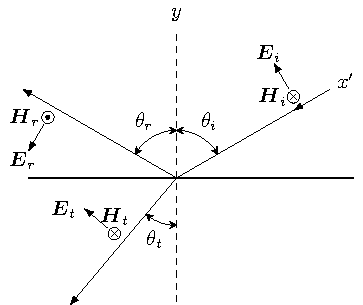
\includegraphics{figObliqueIncidenceParallelElectricFieldReflectedWaveInverted}
\caption{متوازی قطبی موج میں برقی میدان سطح آمد کے متوازی ہوتا ہے۔}
\label{شکل_ترچھی_متوازی_موج}
\end{figure}

مساوات \حوالہ{مساوات_ترچھی_ترچھی_محدد_ایکس_کو_سیدھے_محدد_میں_لکھنا} اور مساوات \حوالہ{مساوات_ترچھی_اکائی_وائے_ڈیش} کی مدد سے شکل \حوالہ{شکل_ترچھی_متوازی_موج} کے لئے
\begin{align}
\kvec{E}_{si}&=(-\cos \theta_i \ax+\sin \theta_i \ay)E_0  e^{j\beta_1 (x\sin \theta_i +y \cos \theta_i)}\\ 
\kvec{H}_{si}&=-\az \frac{E_0}{\eta_1} e^{j\beta_1 (x\sin \theta_i +y \cos \theta_i)}
\end{align}
لکھے جا سکتے ہیں۔اسی طرح گزشتہ معلومات کا سہارا لیتے ہوئے
\begin{align}
\kvec{E}_{sr}&= -(\cos \theta_r \ax+\sin \theta_r \ay)\Gamma_{\parallel} E_0 e^{ j \beta_1 (x \sin \theta_r-y\cos \theta_r)}\\
\kvec{H}_{sr}&=\az\Gamma_{\parallel} \frac{ E_0}{\eta_1} e^{j \beta_1 (x \sin \theta_r-y\cos \theta_r)}\\
\kvec{E}_{st} &= (-\cos \theta_t \ax+\sin \theta_t \ay )\tau_{\parallel} E_0 e^{j \beta_2 (x \sin \theta_t+y\cos \theta_t)}\\
\kvec{H}_{st} &=-\az \tau_{\parallel} \frac{E_0}{\eta_2} e^{j \beta_2 (x \sin \theta_t+y\cos \theta_t)} 
\end{align}
لکھے جا سکتے ہیں۔سرحد \عددیء{(y=0)} پر برقی شرط لاگو کرنے کی خاطر برقی میدان کا وہ حصہ استعمال کیا جائے گا جو سرحد کے متوازی ہے۔یوں \عددیء{\ay} جزو کو رد کیا جائے گا جبکہ \عددیء{\ax} جزو کو استعمال کیا جائے گا لہٰذا
\begin{align*}
-\cos \theta_i \ax E_0  e^{j\beta_1 (x\sin \theta_i +0 \cos \theta_i)}- \cos \theta_r \ax\Gamma_{\parallel} E_0 e^{ j \beta_1 (x \sin \theta_r-0\cos \theta_r)}=-\cos \theta_t \ax\tau_{\parallel} E_0 e^{j \beta_2 (x \sin \theta_t+0\cos \theta_t)}
\end{align*}
یعنی
\begin{align}\label{مساوات_ترچھی_متوازی_قطبی_موج_برقی_شرط}
\cos \theta_i    e^{j\beta_1 x\sin \theta_i}+ \cos \theta_r \Gamma_{\parallel}  e^{ j \beta_1 x \sin \theta_r}=\cos \theta_t \tau_{\parallel}  e^{j \beta_2 x \sin \theta_t}
\end{align}
لکھا جا سکتا ہے۔اس مساوات میں \عددیء{x} کی قیمت تبدیل کرنے سے \عددیء{e} کی طاقت تبدیل ہوتی ہے۔ایسی صورت میں یہ مساوات صرف اور صرف اس صورت درست ہو گا جب مساوات میں تینوں \عددیء{e} کے طاقت، \عددیء{x} کے تمام قیمتوں کے لئے برابر ہوں یعنی
\begin{align}\label{مساوات_ترچھی_متوازی_قطبی_موج_برقی_شرط_پہلا_نتیجہ}
j \beta_1 x\sin \theta_i=j \beta_1 x \sin \theta_r=j \beta_2 x \sin \theta_t
\end{align} 
ہو۔اس مساوات سے
\begin{align}
\theta_i=\theta_r
\end{align}
اور
\begin{align}
\sin \theta_t =\frac{\beta_1}{\beta_2} \sin \theta_i
\end{align}
حاصل ہوتے ہیں جو عین عمودی قطبی موج کے مساوات ہیں۔مساوات \حوالہ{مساوات_ترچھی_متوازی_قطبی_موج_برقی_شرط} میں مساوات \حوالہ{مساوات_ترچھی_متوازی_قطبی_موج_برقی_شرط_پہلا_نتیجہ} پر کرنے سے
\begin{align}\label{مساوات_ترچھی_متوازی_انعکاسی_انحرافی_تعلق_الف}
1   +  \Gamma_{\parallel} =\frac{\cos \theta_t}{\cos \theta_i} \tau_{\parallel} 
\end{align}
حاصل ہوتا ہے۔

سرحد پر مقناطیسی شرط لاگو کرتے ہیں۔چونکہ مقناطیسی میدان سرحد کے متوازی ہے لہٰذا اس کا کوئی جزو رد نہیں کیا جائے گا۔اس طرح
\begin{align*}
-\az \frac{E_0}{\eta_1} e^{j\beta_1 (x\sin \theta_i +0 \cos \theta_i)}+\az \Gamma_{\parallel} \frac{ E_0}{\eta_1} e^{j \beta_1 (x \sin \theta_r-0\cos \theta_r)}=-\az \tau_{\parallel} \frac{E_0}{\eta_2} e^{j \beta_2 (x \sin \theta_t+0\cos \theta_t)} 
\end{align*}
یعنی
\begin{align*}
 e^{j\beta_1 x\sin \theta_i}-\Gamma_{\parallel}  e^{j \beta_1 x \sin \theta_r}= \tau_{\parallel} \frac{\eta_1}{\eta_2} e^{j \beta_2 x \sin \theta_t} 
\end{align*}
لکھا جا سکتا ہے جس میں مساوات \حوالہ{مساوات_ترچھی_متوازی_قطبی_موج_برقی_شرط_پہلا_نتیجہ} پر کرنے سے
\begin{align}\label{مساوات_ترچھی_متوازی_انعکاسی_انحرافی_تعلق_ب}
1-\Gamma_{\parallel} = \tau_{\parallel} \frac{\eta_1}{\eta_2} 
\end{align}
ملتا ہے۔مساوات \حوالہ{مساوات_ترچھی_متوازی_انعکاسی_انحرافی_تعلق_الف} اور مساوات \حوالہ{مساوات_ترچھی_متوازی_انعکاسی_انحرافی_تعلق_ب} حل کرتے ہوئے
\begin{align}\label{مساوات_ترچھی_شرح_انعکاس_متوازی_موج_الف}
\Gamma_{\parallel} =\frac{\eta_2 \cos \theta_t -\eta_1 \cos \theta_i}{\eta_1 \cos \theta_i+\eta_2 \cos \theta_t}
\end{align}
ملتا ہے جو غیر مقناطیسی اور بے ضیاع خطوں میں
\begin{align}\label{مساوات_ترچھی_شرح_انعکاس_بلمقابل_زاویہ_آمد}
\Gamma_{\parallel} =\frac{-\frac{\epsilon_2}{\epsilon_1}\cos \theta_i+\sqrt{\frac{\epsilon_2}{\epsilon_1}-\sin^2 \theta_i}}{\frac{\epsilon_2}{\epsilon_1}\cos \theta_i+\sqrt{\frac{\epsilon_2}{\epsilon_1}-\sin^2 \theta_i}}
\end{align}
صورت اختیار کر لے گی۔اگر خطہ-2 کامل موصل ہو تب \عددیء{\Gamma_{\parallel}=-1} حاصل ہوتا ہے جو متوقع جواب ہے۔ 

متوازی قطبی موج کی صورت میں ایسے آمدی زاویہ ممکن ہے جس پر  \عددیء{\Gamma_{\parallel}=0} حاصل ہو لہٰذا ایسی صورت میں تمام کی تمام موج بغیر انعکاس کے دوسرے خطے میں داخل ہو جاتی ہے۔اس آمدی زاویے کو \اصطلاح{بریوسٹر زاویہ}\فرہنگ{بریوسٹر زاویہ}\فرہنگ{زاویہ!بریوسٹر}\حاشیہب{Brewster angle}\فرہنگ{Brewster angle}\فرہنگ{angle!Brewster} کہتے\حاشیہد{یہ زاویہ سکاٹ لینڈ کے داؤد بریوسٹر کے نام سے  منسوب ہے۔} ہیں۔مساوات \حوالہ{مساوات_ترچھی_شرح_انعکاس_بلمقابل_زاویہ_آمد} کو صفر کے برابر پر کرنے سے زاویہ بریوسٹر 
\begin{align}
\theta_{i,\text{بریوسٹر}} =\sin^{-1} \sqrt{\frac{\frac{\epsilon_2}{\epsilon_1}}{1+\frac{\epsilon_2}{\epsilon_1}}}=\tan^{-1} \sqrt{\frac{\epsilon_2}{\epsilon_1}}
\end{align} 
حاصل ہوتا ہے۔اس مساوات کی دوسری شکل
\begin{align}
\theta_{i,\text{بریوسٹر}}= \sin^{-1} \left(\frac{n_2}{\sqrt{n_1^2+n_2^2}}\right)
\end{align}
ہے۔

کسی بھی موج کو عمودی اور متوازی قطبی امواج کا مجموعہ لکھا جا سکتا ہے۔یوں اگر غیر قطبی موج، سرحد پر  زاویہ بریوسٹر سے آمد ہو تب اس موج کا وہ جزو جو متوازی قطبیت رکھتا ہو سرحد سے مکمل طور دوسری جانب گزر جائے گا جبکہ سرحد سے انعکاسی جزو صرف اور صرف عمودی قطبیت کا ہو گا۔عمودی قطبی موج حاصل کرنے کا یہ آسان طریقہ ہے۔عمودی موج کا کچھ حصہ منعکس ہو گا اور کچھ حصہ منحرف لہٰذا انحرافی موج غیر قطبی ہو گی۔زاویہ بریوسٹر کو \اصطلاح{زاویہ قطبیت}\فرہنگ{زاویہ قطبیت}\فرہنگ{قطبیت!زاویہ}\حاشیہب{polarizing angle}\فرہنگ{angle!polarizing} بھی کہتے ہیں۔  

%==================
\ابتدا{مثال}
ہوا سے شیشے  میں برقی موج بریوسٹر زاویے سے داخل ہوتی ہے جہاں شیشے کا انحرافی مستقل \عددی{n=1.45} ہے۔انحرافی زاویہ حاصل کریں۔

حل:اس شیشے کا بریوسٹر زاویہ
\begin{align*}
\theta_{\text{بریوسٹر}} = \sin^{-1} \frac{1.45}{\sqrt{1+1.45^2}}=55.4^{\circ}
\end{align*}
ہے جسے ابن سھل کے قانون میں استعمال کرتے ہوئے انحرافی زاویہ حاصل کرتے ہیں۔
\begin{align*}
\theta_t=\sin^{-1} \left(\frac{n_1}{n_2} \sin \theta_{\text{بریوسٹر}} \right)=\sin^{-1} \left(\frac{n_1}{\sqrt{n_1^2+n_2^2}}\right)=34.6^{\circ}
\end{align*}

اس مثال میں آپ نے دیکھا کہ \عددی{\sin \theta_t=\cos \theta_{\text{بریوسٹر}}} کے برابر ہے۔یہ ایک عمومی نتیجہ جسے
\begin{align}
\theta_{\text{بریوسٹر}} +\theta_{t}=90^{\circ}
\end{align}
لکھا جا سکتا ہے۔
\انتہا{مثال}
%===================
\ابتدا{مثال}
متوازی قطبی موج ہوا سے پانی کی طرف آمد ہے۔زاویہ بریوسٹر حاصل کریں۔پانی کا جزوی برقی مستقل \عددیء{\epsilon_r=80} لیں۔

حل:
\begin{align}
\theta_{i,\text{بریوسٹر}} =\tan^{-1} \sqrt{\frac{80}{1}}=83.6^{\circ}
\end{align} 
\انتہا{مثال}
%==================
 \ابتدا{مشق}
شکل \حوالہ{شکل_ترچھی_متوازی_موج} میں انعکاسی میدانوں کی سمتیں الٹ تصور کرتے ہوئے شرح انعکاس \عددیء{\Gamma_{\parallel}} حاصل کریں۔چونکہ یہاں انعکاسی میدان الٹ تصور کئے جا رہے ہیں لہٰذا ہم توقع کرتے ہیں کہ \عددیء{\Gamma_{\parallel}} کی حاصل مساوات منفی ایک سے ضرب ہو گی۔

جواب:صرف انعکاسی امواج میں فرق ہو گا جنہیں یوں لکھا جائے گا۔
\begin{align*}
\kvec{E}_{sr}&= (\cos \theta_r \ax+\sin \theta_r \ay)\Gamma_{\parallel} E_0 e^{ j \beta_1 (x \sin \theta_r-y\cos \theta_r)}\\
\kvec{H}_{sr}&=-\az\Gamma_{\parallel} \frac{ E_0}{\eta_1} e^{j \beta_1 (x \sin \theta_r-y\cos \theta_r)}
\end{align*}
شرح انعکاس \عددیء{\frac{\eta_1 \cos \theta_i-\eta_2 \cos \theta_t}{\eta_1 \cos \theta_i+\eta_2 \cos \theta_t}} حاصل ہو گا۔
\انتہا{مشق}
%=====================================
\حصہ{قطبی موج کی ترچھی آمد}
شکل \حوالہ{شکل_قطبی_بیضوی_قطبی_ترچھی_آمد} میں قطبی موج کی ترچھی آمد دکھائی گئی ہے۔اس شکل میں آمدی، انعکاسی اور ترسیلی امواج کے لئے علیحدہ علیحدہ کارتیسی محدد استعمال کئے گئے ہیں۔ان تینوں محدد کے مرکز کو نقطہ \عددی{M} ظاہر کرتی ہے جبکہ تینوں امواج کو اپنے اپنے محدد کے \عددی{x} محدد پر حرکت کرتا تصور کیا گیا ہے۔یوں آمدی موج گھٹتی \عددی{x'} جانب حرکت کر رہی ہے جبکہ انعکاسی موج  بڑھتے \عددی{x''} جانب اور ترسیلی موج بڑھتے \عددی{x'''} جانب حرکت کر رہی ہے۔محدد \عددی{z'}، \عددی{z''} اور \عددی{z'''}،  صفحہ کتاب کے عمودی باہر جانب کو ہے۔یوں ان تینوں کو \عددی{z} سے ظاہر کیا جا سکتا ہے۔آمدی قطبی برقی موج کے عمودی جزو کا حیطہ \عددی{E_{i\perp}} اور دوری زاویہ صفر ہے جبکہ متوازی جزو کا حیطہ \عددی{E_{i\parallel}} اور دوری زاویہ \عددی{\delta_i}  ہے۔ شکل کو دیکھتے ہوئے 
\begin{align}\label{مساوات_ترچھی_بیضوی__قطبی}
\kvec{E}_i&=(E_{i\perp} \az+E_{i\parallel} e^{j\delta_i}\ay')e^{j(\omega t+\beta_1 x')}
\end{align}
لکھا جا سکتا ہے۔انعکاسی مستقل
\begin{align}
\Gamma_{\perp}=\abs{\Gamma_{\perp}} e^{j\phi_{\perp}}\\
\Gamma_{\parallel}=\abs{\Gamma_{\parallel}} e^{j\phi_{\parallel}}
\end{align}
لیتے ہیں۔یوں انعکاسی موج کے  اجزاء 
\begin{align}
E_{r\perp}&=E_z=\Gamma_{\perp} E_{i\perp}=\abs{\Gamma_{\perp}}E_{i\perp} e^{j\phi_{\perp}}\\
E_{r\parallel}&=E_{y''}=\Gamma_{\parallel} E_{i\parallel}e^{j\delta}=\abs{\Gamma_{\parallel}} E_{\parallel} e^{j(\phi_{\parallel}+\delta_i)}
\end{align}
 لکھے جا سکتے ہیں۔اسی طرح  ترسیلی مستقل\حاشیہد{ہم \عددی{\tau} کی علامت موج کے جھکاو جبکہ \عددی{\tau_{\perp}} اور \عددی{\tau_{\parallel}} کو بطور ترسیلی مستقل استعمال کرتے ہیں۔}
\begin{align}
\tau_{\perp}&=\abs{\tau_{\perp}}e^{j\xi_{\perp}}\\
\tau_{\parallel}&=\abs{\tau_{\parallel}}e^{\xi_{\parallel}}
\end{align}
لیتے ہوئے ترسیلی موج کے  اجزاء
\begin{align}
E_{t\perp}&=\tau_{\perp} E_{i\perp}=\abs{\tau_{\perp}} E_{i\perp}e^{j\xi_{\perp}}\\
E_{t\parallel}&=\tau_{\parallel} E_{i\parallel}=\abs{\tau_{\parallel}} E_{i\parallel}e^{j(\xi_{\parallel}+\delta_i)}
\end{align}
ہوں گے۔
\begin{figure}
\centering
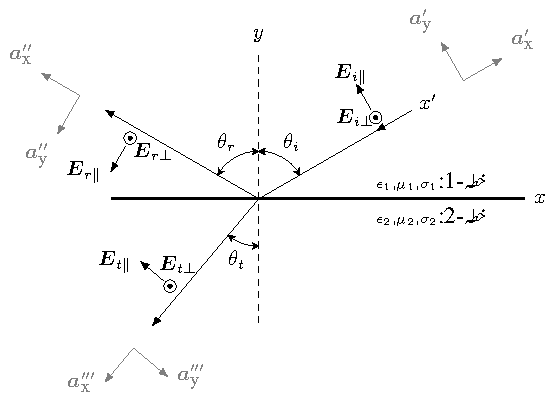
\includegraphics{figObliqueIncidenceEllipticPolarizedElectricWave}
\caption{قطبی برقی موج سرحد پر ترچھی آمد۔}
\label{شکل_قطبی_بیضوی_قطبی_ترچھی_آمد}
\end{figure}
%===============
\ابتدا{مثال}
ہوا سے،  دایاں دائری قطبی موج \عددی{45^{\circ}} کے زاویے سے  کامل موصل سطح پر آمد ہے۔انعکاسی موج کی قطبیت دریافت کریں۔

حل:موصل سطح پر ترچھی آمد دائری قطبی موج کے  انعکاسی مستقل مساوات \حوالہ{مساوات_ترچھی_شرح_انعکاس_عمودی_الف} اور مساوات \حوالہ{مساوات_ترچھی_شرح_انعکاس_متوازی_موج_الف} سے  حاصل کئے جائیں گے۔کامل موصل کی موصلیت \عددی{\sigma \to \infty} لیتے ہوئے  موصل کی قدرتی رکاوٹ \عددی{\eta=\sqrt{\tfrac{j\omega \mu}{\sigma+j\omega \epsilon}}=0} حاصل ہوتی ہے جسے ان مساوات میں پر کرتے ہوئے
\begin{align*}
\Gamma_{\perp}=\Gamma_{\parallel}&=-1
\end{align*}
حاصل ہوتے ہیں۔صفحہ \حوالہصفحہ{مساوات_قطبیت_دائیں_دائری_کوسائن} پر مساوات \حوالہ{مساوات_قطبیت_دائیں_دائری_کوسائن} کی مدد سے منفی \عددی{x'} جانب حرکت کرتی، آمدی دائیں دائری قطبی موج
\begin{align*}
\kvec{E}_i&=E_0[\az\cos(\omega t +\beta x')+\ay' \cos(\omega t +\beta x' -90^{\circ})]
\end{align*}
یعنی
\begin{align*}
\kvec{E}_{si}&=E_0(\az+e^{-j\frac{\pi}{2}} \ay')e^{j\beta_1 x'}
\end{align*}
لکھی جائے گی۔اس موج کو شکل \حوالہ{شکل_قطبیت_الٹ_گھڑی_سے_سمت_گھڑی_قطبیت} میں دکھایا گیا ہے۔ نقطہ \عددی{M} سے دیکھتے ہوئے یہ الٹ گھڑی گھومتی ہے لہٰذا آمدی موج دائیں قطبی ہے۔انعکاسی مستقل استعمال کرتے ہوئے انعکاسی اجزاء 
\begin{align*}
E_{r\perp}&=-E_0\\
E_{r\parallel}&=- E_0 e^{-j\frac{\pi}{2}}
\end{align*}
لکھے جا سکتے ہیں۔یوں مثبت \عددی{x''} جانب حرکت کرتی، انعکاسی موج
\begin{align*}
\kvec{E}_{sr}&=E_0(- \az- e^{-j\frac{\pi}{2}}\ay'')e^{-j\beta_1 x''}
\end{align*}
یعنی
\begin{align*}
\kvec{E}_r=E_0[-\cos (\omega t -\beta x'') \az -\sin(\omega t -\beta x'')\ay'']
\end{align*}
ہو گی.شکل \حوالہ{شکل_قطبیت_الٹ_گھڑی_سے_سمت_گھڑی_قطبیت} میں نقطہ \عددی{R} سے دیکھتے ہوئے انعکاسی موج گھڑی کی سمت میں گھومتی ہے لہٰذا یہ دائری بائیں قطبی ہے۔یوں موصل سطح پر دائیں قطبی موج انعکاس کے بعد بائیں قطبی ہو جاتی ہے۔اسی طرح موصل سطح پر بائیں قطبی موج انعکاس کے بعد دائیں قطبی ہو جاتی ہے۔
\begin{figure}
\centering
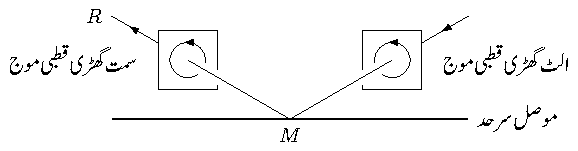
\includegraphics{figObliqueLCRtoRCPonReflectionFromConductor}
\caption{الٹ گھڑی قطبی آمدی موج موصل سطح سے انعکاس کے بعد سمت گھڑی قطبیت رکھتی ہے۔}
\label{شکل_قطبیت_الٹ_گھڑی_سے_سمت_گھڑی_قطبیت}
\end{figure}
\انتہا{مثال}
%===========================

موصل سطح پر صفر برقی میدان پایا جاتا ہے۔شکل \حوالہ{شکل_قطبیت_الٹ_گھڑی_سے_سمت_گھڑی_قطبیت} میں سرحد پر آمدی برقی میدان کے الٹ انعکاسی میدان پیدا ہو کر سرحد پر کل صفر برقی میدان پیدا کرتا ہے۔یوں سرحد پر آمدی اور انعکاسی میدان ایک ہی سمت میں گھومتے ہیں۔یہاں رک کر تسلی کر لیں کہ آپ کو اس بات کی سمجھ آ گئی ہے۔شکل میں آمدی اور انعکاسی امواج کے گھومنے کی سمتیں گول دائروں سے دکھائی گئی ہے۔ان دائروں کو عین سرحد پر تصور کرتے ہوئے غور کریں۔آپ کو سرحد پر دونوں سمتیات ایک ہی سمت میں گھومتے نظر آئیں گے۔   
 
\begin{figure}
\centering
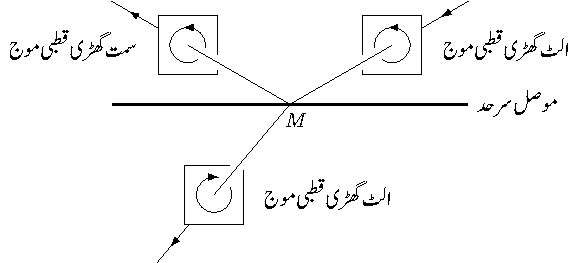
\includegraphics{figObliqueEllipticGeneralCase}
\caption{سرحد پر آمدی، انعکاسی اور ترسیلی برقی سمتیات ایک ہی سمت میں گھومتے ہیں۔}
\label{شکل_قطبیت_عمومی_صورت}
\end{figure}

سرحدی شرائط کے تحت کسی بھی سرحد پر متوازی برقی میدان ہموار پایا جاتا ہے۔اس اصول کر بروئے کار لاتے ہوئے آمدی برقی موج کو دیکھتے ہوئے انعکاسی اور ترسیلی امواج کے گھومنے کی سمت حاصل کی جا سکتی ہے۔ شکل \حوالہ{شکل_قطبیت_عمومی_صورت} میں عمومی صورت حال دکھائی گئی ہے۔آپ دیکھ سکتے ہیں کہ سرحدی شرط پر پورا اترنے کے لئے ضروری ہے کہ آمدی، انعکاسی اور ترسیلی سمتیات سرحد پر ہم قدم ہو کر گھومیں۔ اس طرح ہم کہہ سکتے ہیں کہ بائیں آمدی برقی موج، دائیں انعکاسی اور بائیں ترسیلی برقی امواج پیدا کرے گی جبکہ دائیں آمدی برقی موج، بائیں انعکاسی اور دائیں ترسیلی برقی امواج پیدا کرے گی۔ 

%===========================================
\ابتدا{مثال}
صفحہ \حوالہصفحہ{مثال_مستوی_سمندری_پانی_عمودی_آمد} پر مثال \حوالہ{مثال_مستوی_سمندری_پانی_عمودی_آمد} میں سمندری پانی
 \عددی{(\sigma=5,\mu_R=1,\epsilon_R=78)} پر عمودی آمدی برقی موج کی بات کی گئی۔اسی مثال کو آگے بڑھاتے ہیں۔تصور کریں کہ \عددی{\SI{50}{\mega\hertz}} تعدد کی آمدی بائیں دائری قطبی موج سطح سمندر کے عمود کے ساتھ \عددی{65^{\circ}} کا زاویہ بناتی ہے۔ الف) عمودی اور متوازی انعکاسی مستقل حاصل کریں۔ ب) عمودی اور متوازی ترسیلی مستقل حاصل کریں۔ پ) انعکاسی موج کی قطبیت دریافت کریں۔ ت) آمدی طاقت کا کتنا فی صد سطح پار کرتی ہے۔

حل:سمندری پانی کی قدرتی رکاوٹ
\begin{align*}
\eta_2=\sqrt{\frac{j\omega \mu}{\sigma+j\omega \epsilon}}&=\sqrt{\frac{j 2\pi \times 50\times 10^6\times 4 \pi \times 10^{-7}}{5+j 2\pi\times 50 \times 10^6 \times 78\times 8.85\times 10^{-12}}}\\
&=6.41+j6.14  \quad \si{\ohm}
\end{align*}
اور حرکی مستقل
\begin{align*}
\gamma_2&=\sqrt{j\omega \mu(\sigma+j\omega \epsilon)}\\
&=\sqrt{j 2\pi \times 50\times 10^6\times 4 \pi \times 10^{-7}(5+j 2\pi\times 50 \times 10^6 \times 78\times 8.85\times 10^{-12})}\\
&=30.7+j 32.1 \quad \si{\meter^{-1}}\\
&=\alpha_2+j\beta_2
\end{align*}
ہیں۔ہوا میں طول موج \عددی{\lambda_1=\tfrac{c}{f}=\SI{6}{\meter}} ہے لہٰذا \عددی{\beta_1=\frac{2\pi}{\lambda}=1.047197} ہو گا۔ مساوات \حوالہ{مساوات_ترچھی_عمومی_ابن_سھل} ابن سھل کی عمومی مساوات ہے۔اسے استعمال کرتے ہوئے
\begin{align*}
\sin \theta_t&=\frac{\beta_1}{\beta_2} \sin \theta_i\\
&=\frac{1.047197}{32.1} \sin 65^{\circ}
\end{align*}
سے
\begin{align*}
\theta_t=1.69^{\circ}
\end{align*}
حاصل ہوتا ہے۔یوں مساوات \حوالہ{مساوات_ترچھی_شرح_انعکاس_عمودی_الف} اور مساوات \حوالہ{مساوات_ترچھی_شرح_انعکاس_متوازی_موج_الف} استعمال کرتے ہوئے
\begin{align*}
\Gamma_{\perp}&=\frac{(6.41+j6.14) \cos 65^{\circ} -377 \cos 1.69^{\circ}}{(6.41+j6.14) \cos 65^{\circ} +377 \cos 1.69^{\circ}}\\
&=-0.9856+j0.01359\\
&=0.9857\phase{179.2^{\circ}}
\end{align*}

\begin{align*}
\Gamma_{\parallel} &=\frac{(6.41+j6.14) \cos 1.69^{\circ} -377 \cos 65^{\circ}}{377 \cos 65^{\circ}+(6.41+j6.14) \cos 1.69^{\circ}}\\
&=-0.9199+j0.0712\\
&=0.9227\phase{175.6^{\circ}}
\end{align*}
حاصل ہوتے ہیں۔یوں \عددی{\tau=1+\Gamma} استعمال کرتے ہوئے
\begin{align*}
\tau_{\perp}&=0.0144+j0.01359=0.01979\phase{43.3^{\circ}}\\
\tau_{\parallel}&=0.0801+j0.0712=0.1071\phase{41.6^{\circ}}
\end{align*}
حاصل ہوتا ہے۔

چونکہ عمودی اور متوازی انعکاسی مستقل برابر نہیں ہیں لہٰذا انعکاسی موج بیضوی قطبی ہو گی۔انعکاس کے بعد یہ دائیں قطبی ہو گی۔ترسیلی موج بائیں بیضوی قطبی ہو گی۔

آمدی موج دائری ہے لہٰذا اس میں آدھی طاقت عمودی قطبی اور آدھی متوازی قطبی ہو گی۔یوں کل انعکاسی طاقت، آمدی طاقت کا
\begin{align*}
\frac{\Gamma_{\perp}^2}{2}+\frac{\Gamma_{\parallel}^2}{2}=\frac{0.9857^2}{2}+\frac{0.9227^2}{2}=0.9155
\end{align*}
یعنی \عددی{\SI{91.55}{\percent}} حصہ ہو گا۔بقایا \عددی{\SI{8.4}{\percent}} طاقت ترسیل ہو گا۔
\انتہا{مثال}
%================================
\حصہ{ترسیم ہائی گن}
\اصطلاح{ہائی گن}\فرہنگ{ہائی گن}\فرہنگ{اصول ہائی گن}\حاشیہب{Huygen's principle}\فرہنگ{Huygen's principle} کا اصول کہتا ہے کہ محاذ موج پر ہر نقطے کو منبع کروی موج تصور کیا جا سکتا ہے۔شکل \حوالہ{شکل_ترچھی_ہائی_گن_اصول} میں اس اصول کو دکھایا گیا ہے جہاں ابتدائی محاذ موج پر مختلف نقطوں سے پیدا ثانوی امواج دکھائے گئے ہیں۔یہ ثانوی امواج مل کر ثانوی محاذ موج پیدا کرتی ہیں۔ہائی گن کے اصول کی مدد سے شعاع کی راہ میں حائل چیز کے قریب شعاع کا مڑ جانا سمجھا جا سکتا ہے جو نا تو انعکاس اور نا ہی انحراف کے زمرے میں آتا ہے۔   

\begin{figure}
\centering
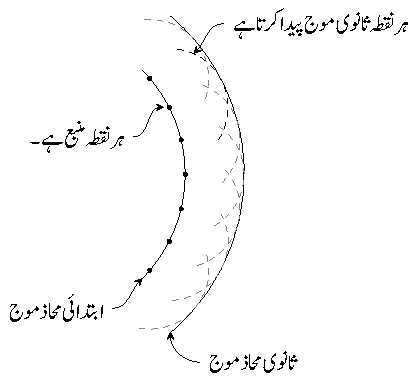
\includegraphics{figObliqueIncidenceHuygensPrinciple}
\caption{ہائی گن کے اصول کے تحت محاذ موج پر ہر نقطہ منبع موج کا کردار ادا کرتا ہے۔}
\label{شکل_ترچھی_ہائی_گن_اصول}
\end{figure}

شعاع کی راہ میں حائل موصل سطح شکل میں دکھائی گئی ہے۔آئیں ہائی گن کے اصول سے نقطہ \عددیء{N} پر برقی میدان 
\begin{align}
E=\int \dif E
\end{align}
حاصل کریں جہاں موصل سطح کے کنارے سے آگے \عددیء{x} محدد پر عمومی نقطے کو منبع موج تصور کرتے ہوئے \عددیء{N} پر میدان \عددیء{\dif E} کے برابر ہے۔
\begin{align}
\dif E=\frac{E_0}{r} e^{-j \beta (r+\delta)} \dif x
\end{align}
سے
\begin{align}
E=\frac{E_0}{r} e^{-j \beta r} \int_a^{\infty} e^{-j \beta \delta} \dif x
\end{align}
لکھا جا سکتا ہے۔اگر \عددیء{\delta \ll r} ہو تب
\begin{align}
\delta=\frac{x^2}{2r}
\end{align}
کے برابر ہو گا۔یوں \عددیء{k^2=\tfrac{2}{r\lambda}} اور \عددیء{u=kx} لیتے ہوئے
\begin{align}
E=\frac{E_0}{k r} e^{-j \beta r} \int_{k a}^{\infty} e^{-j \frac{\pi u^2}{2}} \dif u
\end{align}
لکھا جا سکتا ہے جسے
\begin{align}
E=\frac{E_0}{k r} e^{-j \beta r} \left(\int_0^{\infty} e^{-j \frac{\pi u^2}{2}} \dif u-\int_0^{k a} e^{-j \frac{\pi u^2}{2}} \dif u \right)
\end{align}
لکھ سکتے ہیں۔
%============================
\حصہ{انتشار}
کسی بھی مادہ میں مثبت اور منفی بار قدرتی گھمکی تعدد پر ارتعاش کرتے ہیں۔اس قدرتی گھمکی تعدد یا اس کے قریب تعدد کے موج میں مادہ رکھنے سے ارتعاش زور پکڑتی ہے۔ارتعاش کے حیطے میں اضافے کے لئے درکار توانائی موج سے حاصل کی جاتی ہے۔یوں موج کی طاقت کم ہوتی ہے۔اس طرز کی قوت کے ضیاع کو مخلوط برقی مستقل
\begin{align}
\epsilon=\epsilon'-j \epsilon"=\epsilon_0(\epsilon_R'-j\epsilon_R")
\end{align}
 کی مدد سے ظاہر کیا جا سکتا ہے۔ موج کی تعدد اور مادے کی قدرتی گھمکی تعدد جتنے قریب ہوں، موج اتنی ہی زیادہ طاقت کھوتی ہے۔اس کا مطلب یوں بھی لیا جا سکتا ہے کہ \عددی{\epsilon_R'} اور \عددی{\epsilon_R"} کا دارومدار تعدد پر ہے۔

مقناطیسی موج سے مادے میں طاقت کے ضیاع کو مخلوط مقناطیسی مستقل \عددی{\mu=\mu'-j\mu"} سے ظاہر کیا جاتا ہے۔مقناطیسی اشیاء، مثلاً لوہا، میں ایسا طاقت کا ضیاع نہایت اہمیت رکھتا ہے۔حرکت کرتے موج کے عموماً مسائل میں مقناطیسی موج کی ضیاع قابل نظر انداز ہوتی ہے لہٰذا ایسی صورت میں \عددی{\mu \approx \mu_0} ہی لیا جاتا ہے۔اس کتاب میں ایسا ہی کیا جائے گا۔

ایسا مادہ جس کے مستقل \عددی{\epsilon=\epsilon'-j\epsilon"} اور \عددی{\mu = \mu_0} ہوں کی قدرتی رکاوٹ صفحہ \حوالہصفحہ{مساوات-موج_قدرتی_رکاوٹ} پر مساوات \حوالہ{مساوات-موج_قدرتی_رکاوٹ} سے
\begin{align}
\eta=\sqrt{\frac{j \omega \mu_0}{j \omega (\epsilon'-j\epsilon")}}=\sqrt{\frac{j\omega \mu_0}{\omega \epsilon"+j\omega \epsilon'}}
\end{align}
لکھی جا سکتی ہے۔اس مساوات میں حقیقی جزو \عددی{\omega \epsilon"} ہے جو طاقت کے ضیاع کی وجہ بنتا ہے لہٰذا 
\begin{align}
\omega \epsilon"=\sigma
\end{align}
لکھا جا سکتا ہے جہاں موصلیت طاقت کے ضیاع کا جزو ہے۔اسی طرح مساوات \حوالہ{مساوات_موج_حرکی_مستقل_الف} کو یوں
\begin{align}
\gamma=\mp \sqrt{j \omega \mu  \left[j \omega (\epsilon'-j\epsilon" )\right]}=\mp \sqrt{j \omega \mu  \left(\omega \epsilon"+j\omega\epsilon' \right)}
\end{align}
لکھا جا سکتا ہے۔یہاں بھی \عددی{\sigma=\omega\epsilon"} لکھ کر ضیاعی جزو کی نشاندہی کی جا سکتی ہے۔

آئیں اب اصل موضوع کی بات کریں۔چونکہ برقی مستقل کا دارومدار موج کی تعدد پر ہے لہٰذا تعدد تبدیل  کرنے سے برقی مستقل بھی تبدیل ہو گا۔برقی مستقل تبدیل کی تبدیلی سے انحرافی مستقل\فرہنگ{انحرافی مستقل}\حاشیہب{refractive index}\فرہنگ{refractive index} بھی تبدیل ہوتا ہے۔مختلف تعدد کے امواج کو درپیش مختلف انحرافی مستقل ہی استعمال کرتے ہوئے شیشے کا  \اصطلاح{منشور}\فرہنگ{منشور}\حاشیہب{prism}\فرہنگ{prism} سفید شعاع کے رنگ علیحدہ علیحدہ کرتا ہے۔شکل \حوالہ{شکل_ترچھی_انتشار_بذریعہ_منشور} میں ایسا دکھایا گیا ہے۔رنگ علیحدہ کرنے کے عمل کو \اصطلاح{زاویائی انتشار}\فرہنگ{زاویائی!انتشار}\فرہنگ{انتشار!زاویائی}\حاشیہب{angular dispersion}\فرہنگ{angular dispersion}\فرہنگ{dispersion!angular} یا \اصطلاح{رنگین انتشار}\فرہنگ{رنگین انتشار}\فرہنگ{انتشار!رنگین}\حاشیہب{chromatic dispersion}\فرہنگ{dispersion!chromatic} کہتے ہیں۔

\begin{figure}
\centering
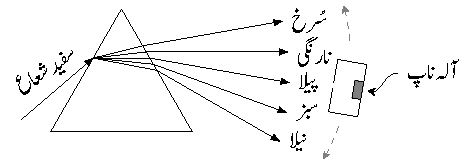
\includegraphics{figObliquePrism}
\caption{شعاع کی انتشار سے منشور سفید شعاع کے رنگ بکھیرتا ہے۔}
\label{شکل_ترچھی_انتشار_بذریعہ_منشور}
\end{figure}
یہاں انتشار سے مراد، موج کے قابل شناخت حصوں کو علیحدہ کرنا ہے۔شعاع کے قابل شناخت اجزاء اس کے مختلف رنگ ہیں۔منشور شعاع کے رنگ علیحدہ علیحدہ کرتا ہے۔یہاں اہم نتیجہ یہ ہے کہ منشور نے شعاع کی طاقت کو تعدد کی نسبت سے مختلف حصوں میں بانٹ دیا ہے۔فرض کریں کہ ہم کسی شعاع میں سبز اور نیلے رنگ کی مقدار جاننا چاہتے ہیں۔شعاع کی طاقت ناپنے کا آلہ منشور کے سامنے سبز اور نیلے شعاع کی مقام پر رکھتے ہوئے ان کی طاقت ناپی جائے گی۔سفید شعاع کی طاقت بھی ناپی جائے گی۔جیسے شکل میں دکھایا گیا ہے، آلہ ناپ تک شعاع ڈبے میں باریک سوراخ کے ذریعہ پہنچتی ہے۔آلہ ناپ شعاع کے ان تمام حصوں کی طاقت ناپے گا جو سوراخ سے گزر پائیں۔یوں سوراخ جتنا چھوٹا ہو، آلہ ناپ تک پہنچتی \اصطلاح{شعاعی پٹی}\فرہنگ{شعاعی پٹی}\فرہنگ{پٹی!شعاعی}\حاشیہب{spectral packet}\فرہنگ{spectral packet} میں تعددی فرق اتنی کم پائی جائے گی۔یوں سوراخ چھوٹے سے چھوٹا کرتے ہوئے کسی بھی تعدد کی طاقت بہتر سے بہتر ناپی جا سکتی ہے۔ہم شعاع کو تصوراتی طور پر شعاعی پٹیوں کا مجموعہ تصور کرتے ہیں۔

آئیں اب ایسی غیر مقناطیسی مادے کی بات کریں جس کا انحرافی مستقل تعدد کے ساتھ تبدیل ہوتا ہو۔ایسے خطے میں مستوی موج کا حرکی مستقل
\begin{align}
\beta(\omega)=\omega\sqrt{\mu_0 \epsilon\left(\omega\right)}=n(\omega)\frac{\omega}{c}
\end{align}
صورت اختیار کرے گا جہاں \عددی{\epsilon(\omega)} اور \عددی{n(\omega)} لکھ کر اس حقیقت کی نشاندہی کی گئی ہے کہ برقی مستقل اور انحرافی مستقل تعدد پر منحصر ہیں۔اگر تعدد بڑھانے سے انحرافی مستقل \عددی{n} بھی بڑھے تب \عددی{\beta(\omega)} بالمقابل \عددی{\omega} کی صورت شکل \حوالہ{شکل_ترچھی_حرکی_مستقل_بالمقابل_تعدد_خط} کے طرز پر ہو گی۔
\begin{figure}
\centering
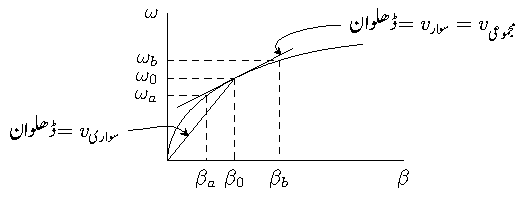
\includegraphics{figObliqueDispersionCurve}
\caption{زاویائی مستقل بالمقابل تعدد۔تعدد \عددی{\omega_0} پر خط کے مماس کی ڈھلوان مجموعی رفتار دیتا ہے جبکہ محدد کے مرکز سے اس نقطے تک خط کی ڈھلوان دوری رفتار ہے۔}
\label{شکل_ترچھی_حرکی_مستقل_بالمقابل_تعدد_خط}
\end{figure}

فرض کریں کہ شکل \حوالہ{شکل_ترچھی_حرکی_مستقل_بالمقابل_تعدد_خط} ایسی خطے کو ظاہر کرتی ہے جس میں \عددی{\omega_a} اور \عددی{\omega_b} تعدد کے امواج پائے جاتے ہیں۔دونوں  امواج \عددی{x} خطی قطبی ہیں اور بڑھتے \عددی{z} جانب حرکت کر رہے ہیں۔دونوں کا حیطہ برابر ہے۔ان کا مجموعی میدان
\begin{align}\label{مساوات_ترچھی_انتشار_الف}
E_{\text{مجموعہ}}=E_0\left[e^{-j \beta_a z}e^{j \omega_a t}+e^{-j \beta_b z}e^{j \omega_b t}\right]
\end{align}
ہو گا جو علیحدہ علیحدہ میدانوں کا سادہ مجموعہ ہے۔یاد رہے کہ ان امواج کی تعدد مختلف ہے لہٰذا مجموعی دوری مساوات لکھتے ہوئے تعدد کو مد نظر رکھنا ضروری ہے۔شکل \حوالہ{شکل_ترچھی_حرکی_مستقل_بالمقابل_تعدد_خط} کو دیکھتے ہوئے
\begin{align}
\Delta \omega&=\omega_0-\omega_a=\omega_b-\omega_0\\
\Delta \beta&\approx\beta_0-\beta_a\approx\beta_b-\beta_0
\end{align}
لکھا جا سکتا ہے جہاں دیے امواج کی اوسط تعدد \عددی{\beta_0} کی نشاندہی بھی کی گئی ہے۔اگر دونوں امواج کے تعدد میں فرق کم ہو تب نقطہ  \عددی{\omega_0} پر شکل \حوالہ{شکل_ترچھی_حرکی_مستقل_بالمقابل_تعدد_خط} کے خط کو یہاں کے مماس سے ظاہر کیا جا سکتا ہے۔ایسی صورت میں مندرجہ بالا  \عددی{\Delta \beta} کی مساوات میں \عددی{\approx} کو \عددی{=} لکھا جا سکتا ہے۔مندرجہ بالا دو مساوات استعمال کرتے ہوئے مساوات \حوالہ{مساوات_ترچھی_انتشار_الف} کو
\begin{gather}
\begin{aligned}
E_{\text{مجموعی}}&=E_0 e^{-j \beta_0 z} e^{j \omega_0 t}\left[e^{j \Delta \beta z} e^{-j \Delta \omega t}+e^{-j \Delta \beta z} e^{j \Delta \omega t}\right]\\
&=2 E_0 e^{j(\omega_0 t -\beta_0 z)} \cos(\Delta \omega t-\Delta \beta z)
\end{aligned}
\end{gather}
 لکھا جا سکتا ہے۔اس سے حقیقی موج کی مساوات
\begin{align}
E_{}(z,t)=2 E_0 \cos(\Delta \omega t-\Delta \beta z) \cos (\omega_0 t -\beta_0 z)
\end{align}
لکھی جا سکتی ہے۔

%=================================
\newpage
\حصہء{سوالات}

%=================
\ابتدا{سوال}
دائیں دائری قطبی موج  نیم لامحدود پلیکسی گلاس  \عددی{(\sigma=0,\mu_R=1,\epsilon_R=3.45)} کی سطح پر بریوسٹر زاویے سے آمد ہے۔آمدی کثافت طاقت \عددی{\SI{100}{\watt\per\meter\squared}} ہے۔الف) پلیکسی گلاس کا بریوسٹر زاویہ حاصل کریں۔ ب) \عددی{\Gamma_{\parallel}} اور \عددی{\Gamma_{\perp}} حاصل کریں۔ پ) انعکاسی اور ترسیلی کثافت طاقت دریافت کریں۔ ت) انعکاسی اور ترسیلی امواج کی قطبیت بیان کریں۔ (آمدی دائری قطبی موج میں آدھی طاقت عمودی برقی اور آدھی طاقت متوازی برقی ہو گی۔)

جوابات:\عددی{61.7^{\circ}}، \عددی{\Gamma_{\parallel}=0}، \عددی{\Gamma_{\perp}=-0.549}، \عددی{\SI{15}{\watt\per\meter\squared}}، \عددی{\SI{85}{\watt\per\meter\squared}}، انعکاسی موج خطی قطبی جبکہ ترسیلی موج بیضوی قطبی ہے۔
\انتہا{سوال}
%=================
\ابتدا{سوال}
شکل \حوالہ{شکل_ترچھی_شیش_ریشہ} میں شیش ریشہ دکھایا گیا ہے۔اس شیش ریشے میں بائیں جانب سے شعاع \عددی{\theta} زاویے سے داخل ہوتی ہے۔یہ شعاع غلاف سے مکمل اندرونی انعکاس کرتے ہوئے شیش ریشے کے دوسرے سر تک پہنچتی ہے۔بیرونی خلاء کا انحرافی مستقل \عددی{n_0=1} لیتے ہوئے \عددی{\theta} کی وہ حد دریافت کریں جس کے اندر رہتے ہوئے  شیش ریشے میں مکمل اندرونی انعکاس پائی جائے گی۔\عددی{\sin \theta} کو شیش ریشے کی \اصطلاح{عددی شگاف}\فرہنگ{عددی شگاف}\حاشیہب{numerical aperture}\فرہنگ{numerical aperture} کہتے ہیں۔   
\begin{figure}
\centering
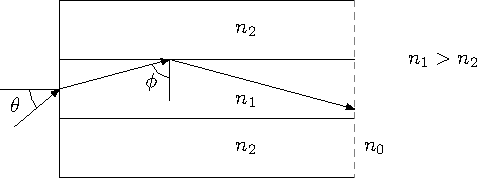
\includegraphics{figObliqueOpticalFiber}
\caption{شیش ریشہ۔}
\label{شکل_ترچھی_شیش_ریشہ}
\end{figure}

جواب:\عددی{\theta_{\text{بلندتر}}=\sin^{-1} \sqrt{n_1^2-n_2^2}}
\انتہا{سوال}
%=======================
\ابتدا{سوال}
شکل \حوالہ{شکل_ترچھی_شیش_ریشہ} میں \عددی{\theta} بریوسٹر زاویہ اور \عددی{\phi} زاویہ فاصل ہونے کی صورت میں \عددی{n_0} کو \عددی{n_1} اور \عددی{n_2} کی صورت میں بیان کریں۔

جواب:\عددی{n_0=\frac{n_1}{n_2}\sqrt{n_1^2-n_2^2}}
\انتہا{سوال}
%=====================
\ابتدا{سوال}
ایسا منشور جو  متوازی برقی موج کو بغیر گھٹائے گزرنے دے \اصطلاح{بریوسٹر منشور}\فرہنگ{منشور!بریوسٹر}\حاشیہب{Brewster prism}\فرہنگ{prism!Brewster} کہلاتا ہے۔ شکل \حوالہ{شکل_ترچھی_منشور} میں دکھائے منشور کو \عددی{n=1.45} کے شیشے سے بنایا گیا ہے۔اس شکل میں دکھائی گئی صورت حال کو دیکھتے ہوئے زاویہ \عددی{\alpha} حاصل کریں۔ (داخلی اور خارجی شعاع شیشے کے عمود کے ساتھ بریوسٹر زاویہ بناتے ہیں۔اس سے انعکاسی ضیاع کا خاتمہ حاصل کیا جاتا ہے۔)
\begin{figure}
\centering
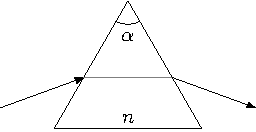
\includegraphics{figObliquePrismBrewster}
\caption{منشور}
\label{شکل_ترچھی_منشور}
\end{figure}

جواب:یہاں منشور کے اندر شعاع، منشور کے قاعدے کے متوازی ہے۔ \عددی{\alpha=69.2^{\circ}}
\انتہا{سوال}
%=====================
\ابتدا{سوال}
شکل \حوالہ{شکل_ترچھی_منشور} میں دکھائے گئے بریوسٹر منشور میں عمودی برقی موج کا کتنا فی صد گزر پائے گا۔

جواب:\عددی{\SI{76}{\percent}}
\انتہا{سوال}
%======================
\ابتدا{سوال}
شکل \حوالہ{شکل_ترچھی_منشور_سمت_تبدیل} میں شعاع کی سمت \عددی{90^{\circ}} تبدیل کرنے کی خاطر منشور استعمال کیا گیا ہے۔انعکاسی ضیاع سے چھٹکارے کی خاطر منشور کے بائیں اور بالائی سطحوں پر انعکاس مخلاف تہہ چڑھائی گئی ہے۔منشور کو خالی خلاء میں استعمال کرنے کی خاطر \عددی{n_1} کی کم سے کم قیمت دریافت کریں۔ 
\begin{figure}
\centering
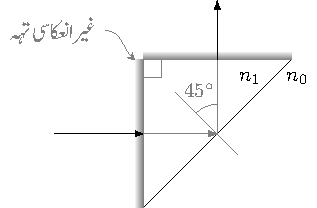
\includegraphics{figObliquePrismNintyDegreeReflection}
\caption{منشور سے شعاع کی سمت تبدیل کی جا سکتی ہے}
\label{شکل_ترچھی_منشور_سمت_تبدیل}
\end{figure}

جواب:\عددی{n_1>1.41}

\انتہا{سوال}
%=============================
\ابتدا{سوال}
دائری قطبی برقی موج دو عدد خطی قطبی امواج کے مجموعے سے بنی ہوئی ہے۔خطی قطبی امواج \عددی{E_x=5\cos(\omega t -\beta z)} اور \عددی{E_y=5\cos(\omega t -\beta z -90^{\circ})} ہیں۔ یہ دائری قطبی موج خطہ-1 \عددی{(\mu_{R1}=1, \epsilon_{R1}=1)} سے خطہ-2  \عددی{(\mu_{R2}=1, \epsilon_{R2}=3.5)} کے سرحد پر \عددیء{45^{\circ}} زاویے سے  پہنچتی ہے۔زاویہ سرحد کے عمود کے ساتھ ناپا جاتا ہے۔انعکاسی موج کی شرح رداس حاصل کریں۔

جواب:\عددی{2.38}
\انتہا{سوال}
%==================================
\ابتدا{سوال}
دائری قطبی برقی موج خطہ-1 \عددی{(\mu_{R1}=1, \epsilon_{R1}=1)} سے خطہ-2  \عددی{(\mu_{R2}=1, \epsilon_{R2}=4)} کے سرحد پر \عددی{\theta} زاویے سے  پہنچتی ہے۔زاویہ سرحد کے عمود کے ساتھ ناپا جاتا ہے۔ انعکاسی موج کی شرح رداس مندرجہ ذیل صورتوں میں حاصل کریں۔ الف) \عددی{\theta=30^{\circ}}،
 ب)\عددی{\theta=60^{\circ}}، پ) \عددی{\theta=63.43^{\circ}}

جواب:\عددی{1.35}، \عددی{10.9}، \عددی{7409}
\انتہا{سوال}
%=============================
\ابتدا{سوال}
دائیں بیضوی قطبی برقی موج از خود عمودی قطبی موج  \عددی{E_x=8\cos(\omega t -\beta z)} اور متوازی قطبی موج \عددی{E_y=6\cos(\omega t -\beta z -90^{\circ})}  کا مجموعہ ہے۔یہ دائیں بیضوی قطبی موج خطہ-1 \عددی{(\mu_{R1}=1, \epsilon_{R1}=1)} سے خطہ-2  \عددی{(\mu_{R2}=1, \epsilon_{R2}=3)} کے سرحد \عددی{z=0} پر \عددیء{30^{\circ}} زاویے سے  پہنچتی ہے۔زاویہ سرحد کے عمود کے ساتھ ناپا گیا ہے۔انعکاسی موج کی شرح رداس حاصل کریں۔

جواب:\عددی{2.68}
\انتہا{سوال}
%==================================

\ابتدا{سوال}
دائیں بیضوی قطبی برقی موج از خود عمودی قطبی موج  \عددی{E_x=8\cos(\omega t -\beta z)} اور متوازی قطبی موج \عددی{{E_y=6\cos(\omega t -\beta z -90^{\circ})}}  کا مجموعہ ہے۔یہ دائیں بیضوی قطبی موج خطہ-1 \عددی{(\mu_{R1}=1, \epsilon_{R1}=1)} سے خطہ-2  \عددی{(\mu_{R2}=1, \epsilon_{R2}=3)} کے سرحد \عددی{z=0} پر \عددیء{60^{\circ}} زاویے سے  پہنچتی ہے۔زاویہ سرحد کے عمود کے ساتھ ناپا گیا ہے۔انعکاسی موج کی شرح رداس حاصل کریں۔اس کی قطبیت بھی دریافت کریں۔

جواب:شرح رداس لامحدود ہے۔موج عمودی قطبی ہے۔
\انتہا{سوال}
%==================================
